\section[Online/Real-time Analysis]{Online Analysis}
\label{sec:online}

On similar lines as \cite{ghanvati01, sanchez01}, test were conducted for checking if the symptoms of Critical Slowing Down could  be detected by a real-time/online analysis of the state variables of a power grid. In other words, can computing the autocorrelation and variance of real-time PMU data processed over a running window function appropriately as Early Warning Signs of an impending approach instability.

Bifurcation Theory states that a small change in system parameters, such the governor reference power for a generator ($P_{Gen}$) at certain points, can lead to major upsets in the stability of the power grid. We ran a simulation in which a system was purposefully stressed (via a near constant linear load increment) as time progressed but many restrictions/safety mechanisms were lifted with the aim of singling-out the cause of bifurcation to a change in $P_{Gen}$(s), in order to best demonstrate that the proposed statistical mechanisms (computing autocorrelations and variances) function well as Early Warning Signs even for slow and steady variations of loads, and not just for sudden changes in state variables caused due to reactionary corrective protection mechanisms or the machines not being given `free-range' for chasing load increments due to specified safety limits on maximum allowed generated powers. Below is the set of special conditions used for the simulation of the IEEE 9 Bus system:

\textbf{Steps and Conditions for Simulating the IEEE 9 Bus System towards instability:}

\begin{enumerate}
	\item The three load points of the system (Buses 5, 6 and 8) were linearly increased in time, at a rate of $\Delta P \%$ per minute plus a small white noise component $\mathcal{N}(0, \sigma_v)$, with every increment happening at $\Delta t$ time intervals. 
	\begin{equation}
		P_{L_i}(t+\Delta t) = P_{L_i}(t)*\left(1+ \frac{\Delta P_{L_i}}{100}\right) + \mathcal{N}(0, \sigma_v)
	\end{equation} 
	Here, $\Delta P_{L}$ values were assigned randomly between $8-12\%$ for every load bus, $\sigma_v = 0.01$ and $\Delta t = 0.1$ seconds.
	\item Simulation ODE solver solves for the new state variables for the system every $0.01$ seconds or $t_{sampling}=0.01$ seconds. This means that the simulation output can be likened to a stream of PMU data whose sampling rate is $100$ Hz or $f_{sampling} = 100$ Hz.
	\item Protection mechanisms were disabled. No remedial/corrective action was taken for any drop in bus voltages/grid frequency or any increase in line currents/MVAs.
	\item `Dummy' governors were placed on the three generators (at buses 1, 2 and 3) which could respond instantly to load changes by changing the set reference generation powers $P_{Gen}$(s) with zero time lag.
	\item The generator limits for $P_{Gen_{MAX}}$, $Q_{Gen_{MAX}}$, etc. were removed. Thus the generators had complete freedom to `chase' the load increments at the load buses, including factoring in the extra line-losses.
\end{enumerate} 

Based on the above conditions, simulations were run in PSSE. The simulations ran for about two minutes before the grid `blacked out' i.e. PSSE solver returned the message `Network Not Converged' as the continuously increasing loads could not be handled by the generators while maintaining synchronism. The outputs of the state variables, including Demand/Load Powers, Generated Powers, Bus Frequencies, Bus Voltages, Line Currents and Line MVAs have been presented below in Figure \ref{fig:psse_run02}.

\begin{figure}[!ht]
	\centering
	\begin{subfigure}{\textwidth}
		\centering
		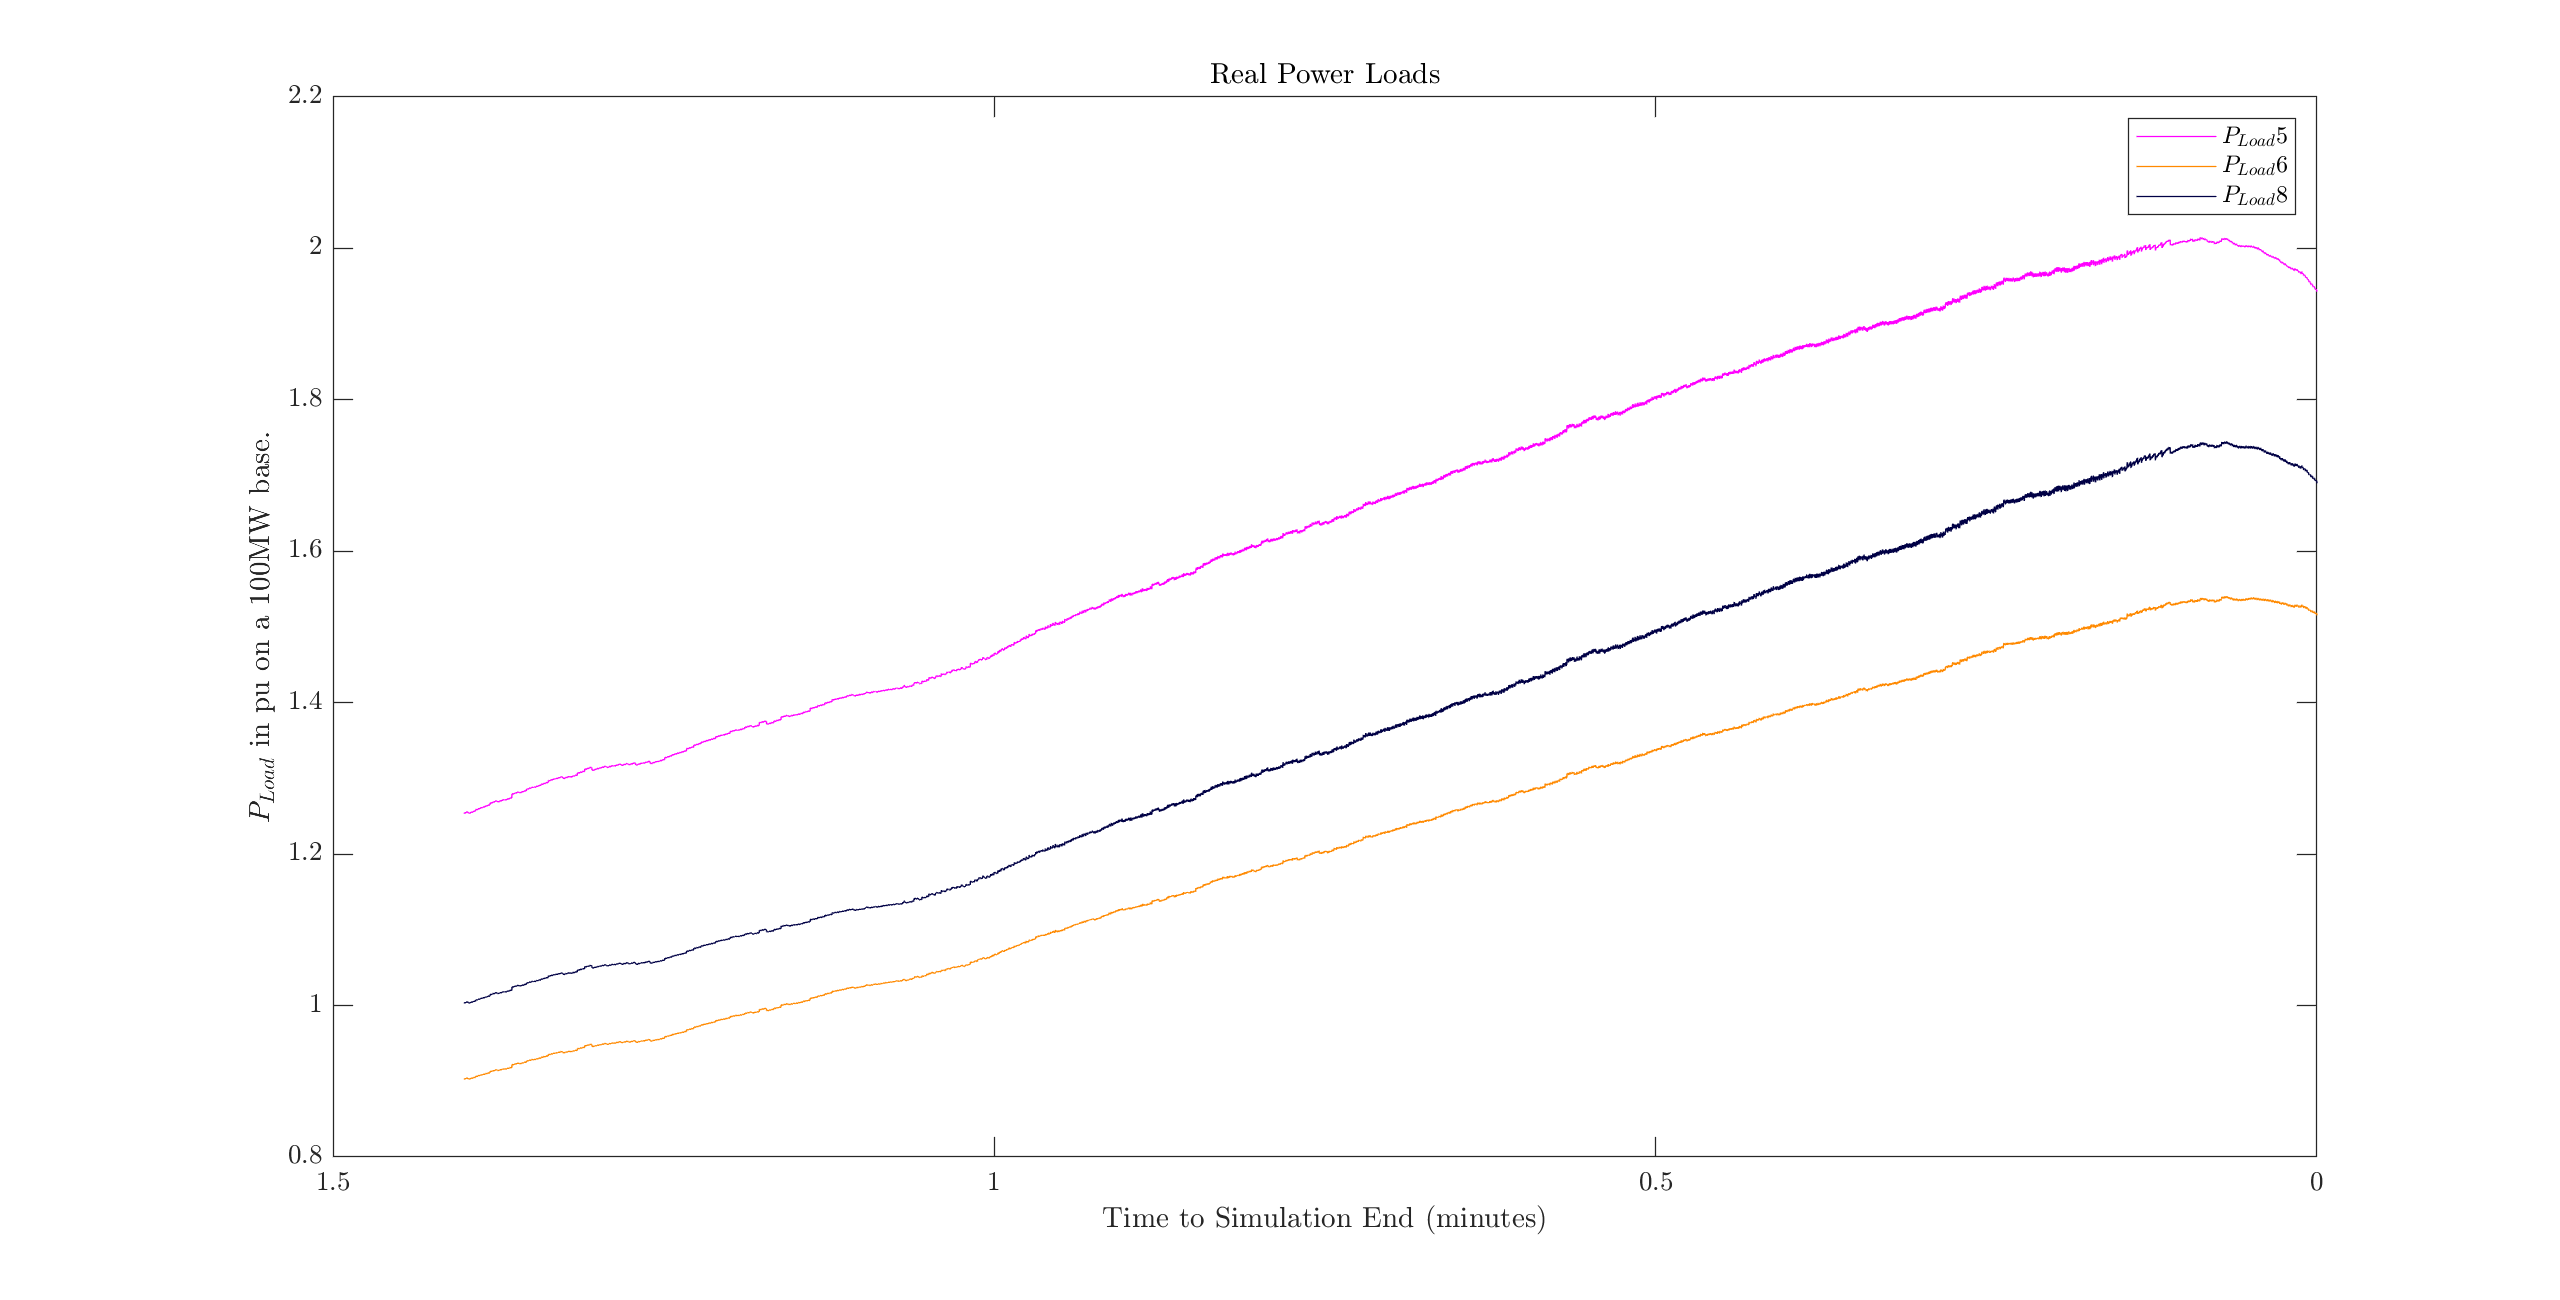
\includegraphics[scale=0.25]{../figures/analysis_matlab/ploads_run02}
		\caption{Real Power Loads for the simulated IEEE 9 Bus System vs simulation time.}
	\end{subfigure}
	
	\begin{subfigure}{\textwidth}
		\centering
		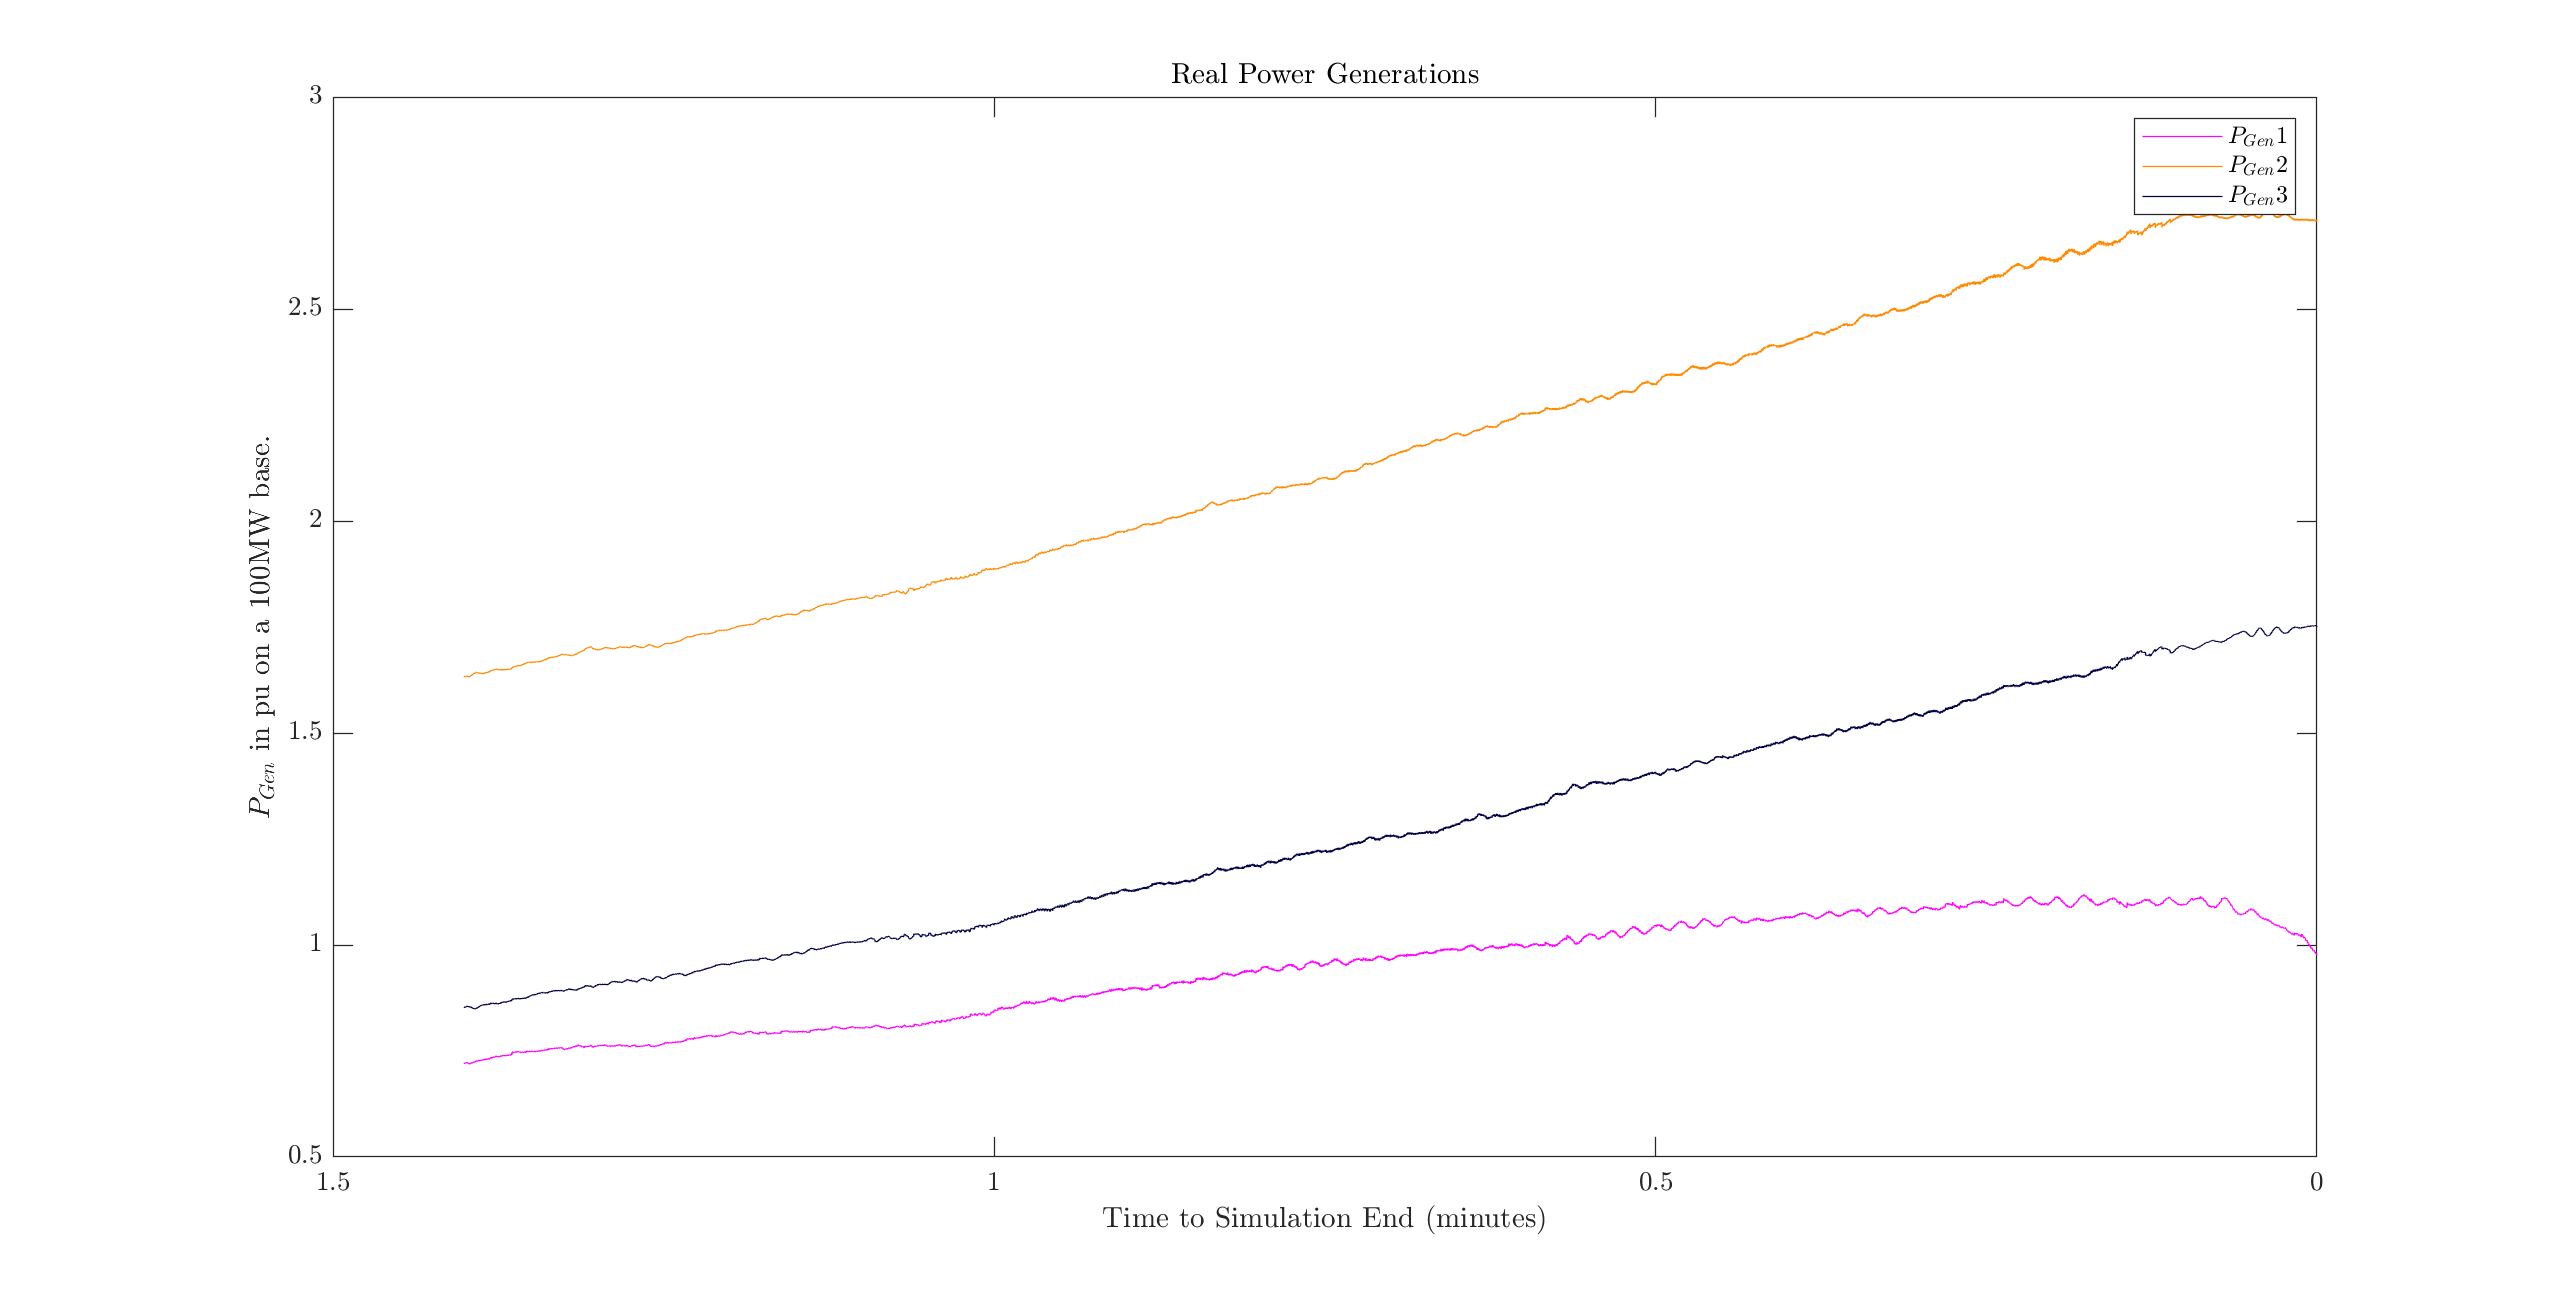
\includegraphics[scale=0.25]{../figures/analysis_matlab/pgens_run02}
		\caption{Generated Real Powers for the simulated IEEE 9 Bus System vs simulation time.}
	\end{subfigure}

	\caption{Simulation results of the IEEE 9 Bus System as per the prescribed conditions.}
	\label{fig:psse_run02}
\end{figure}

\begin{figure}[!htpb]
	\centering
	\begin{subfigure}{\textwidth}
		\centering
		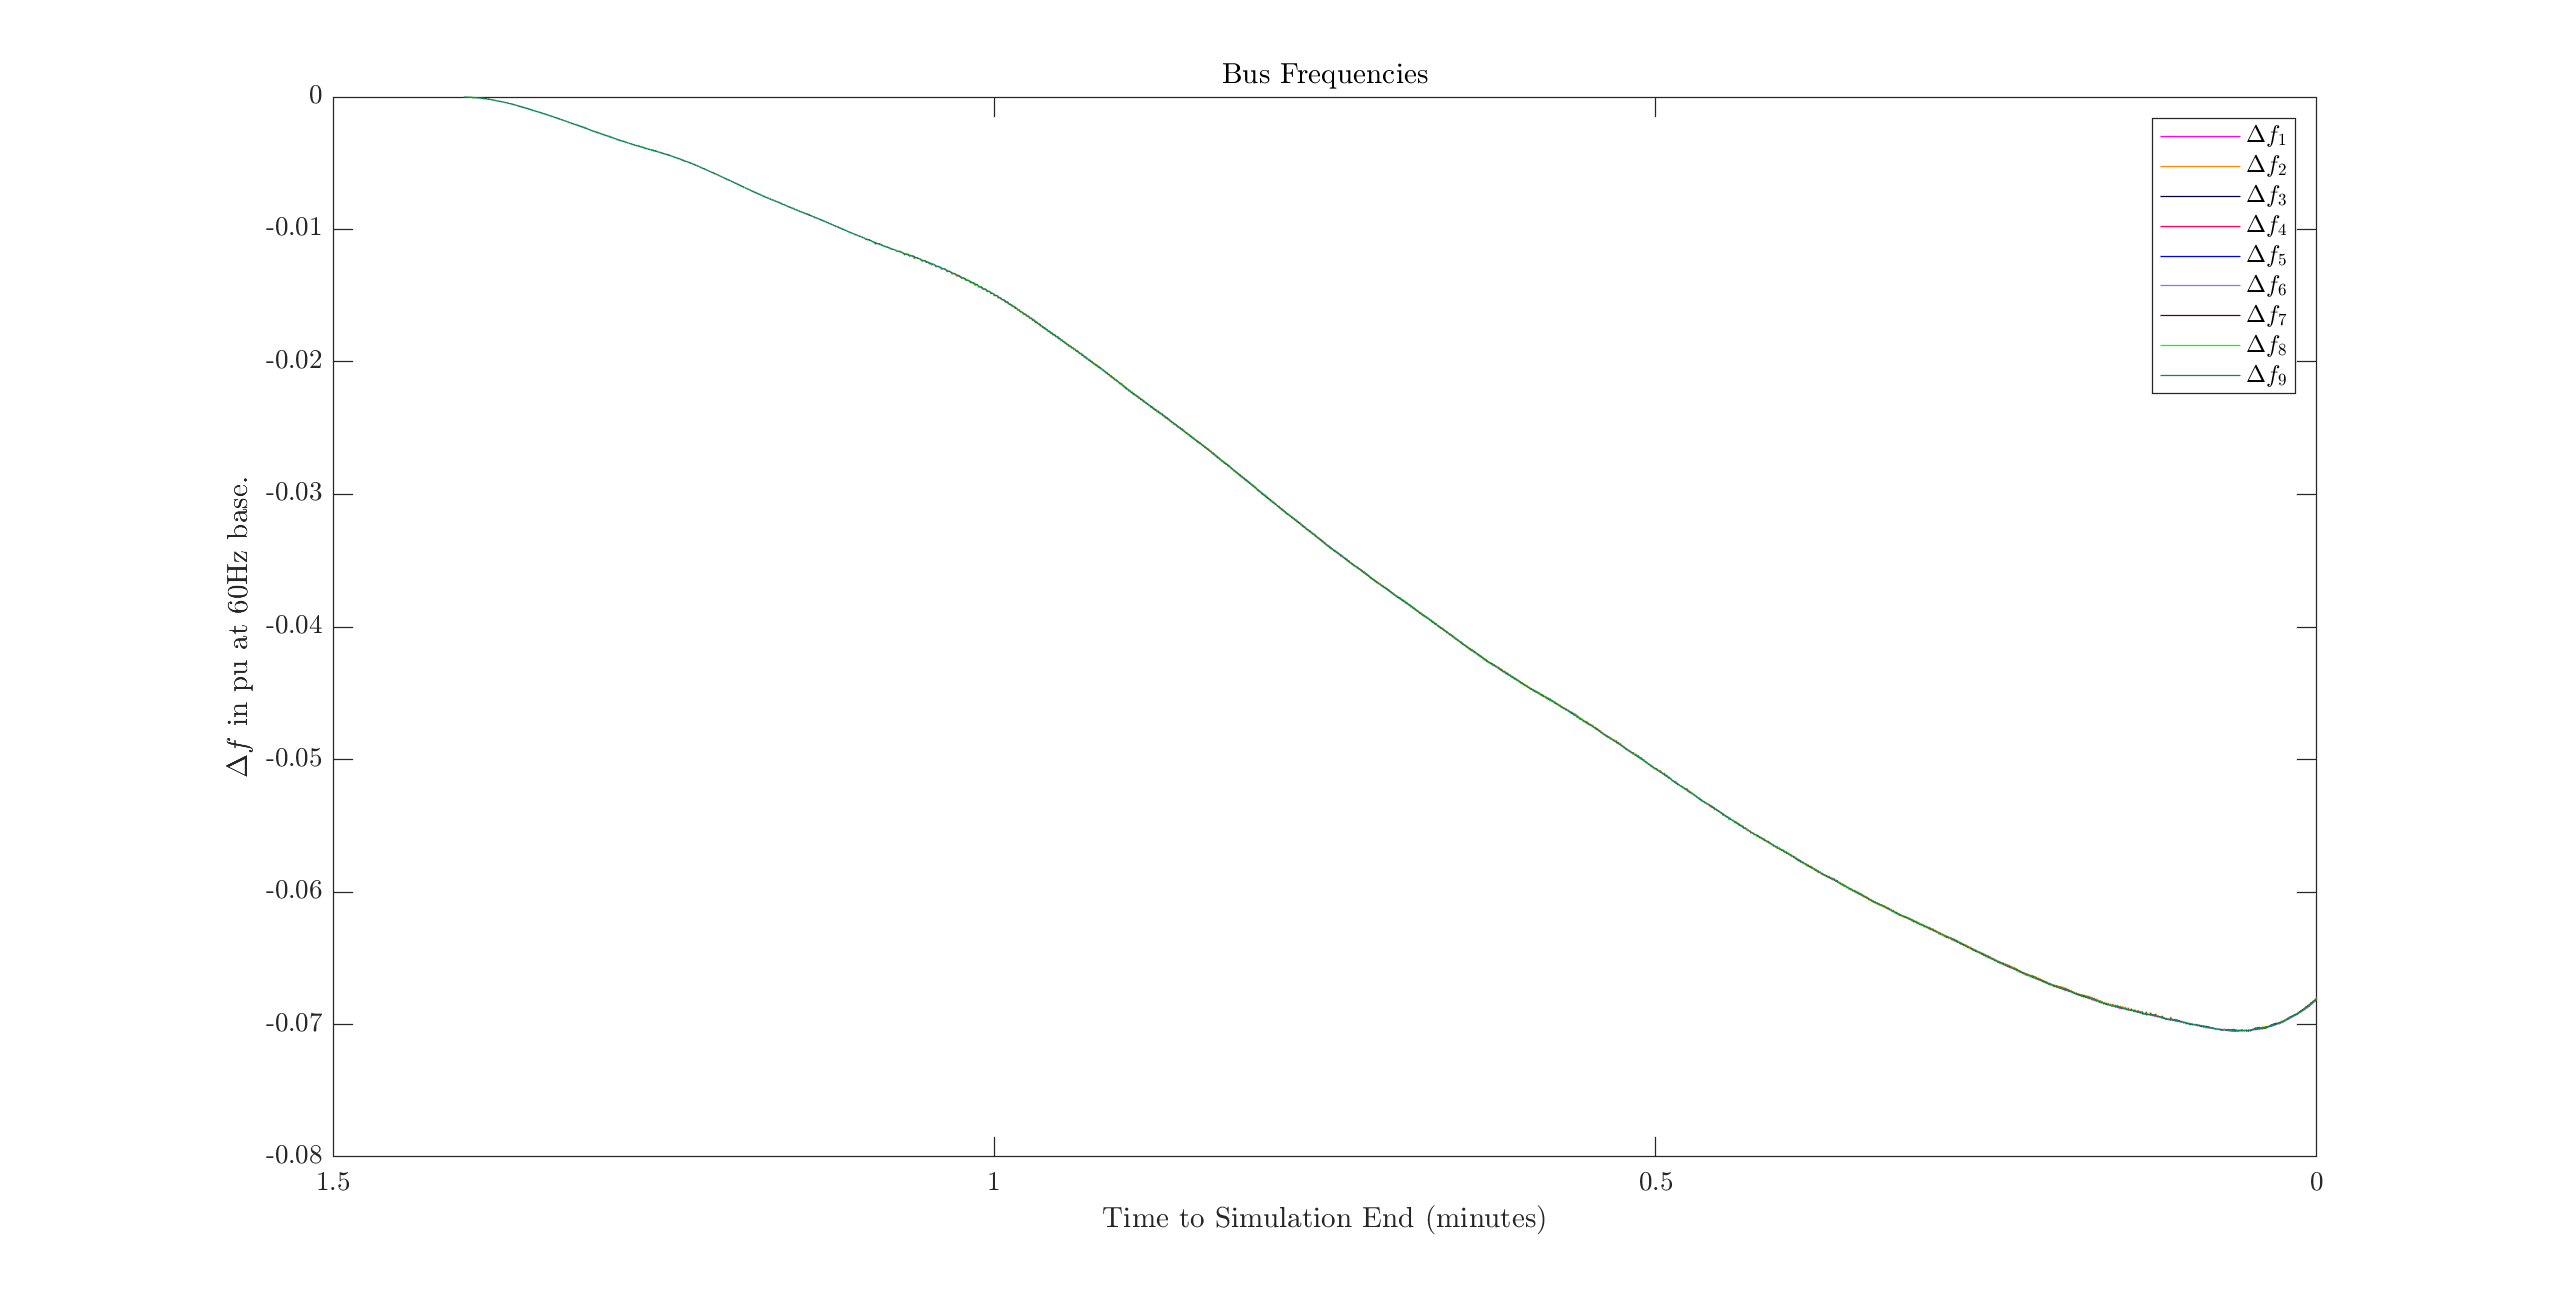
\includegraphics[scale=0.25]{../figures/analysis_matlab/frequencies_run02}
		\caption{Bus Frequencies for the simulated IEEE 9 Bus System vs simulation time.}
	\end{subfigure}
	
	\begin{subfigure}{\textwidth}
		\centering
		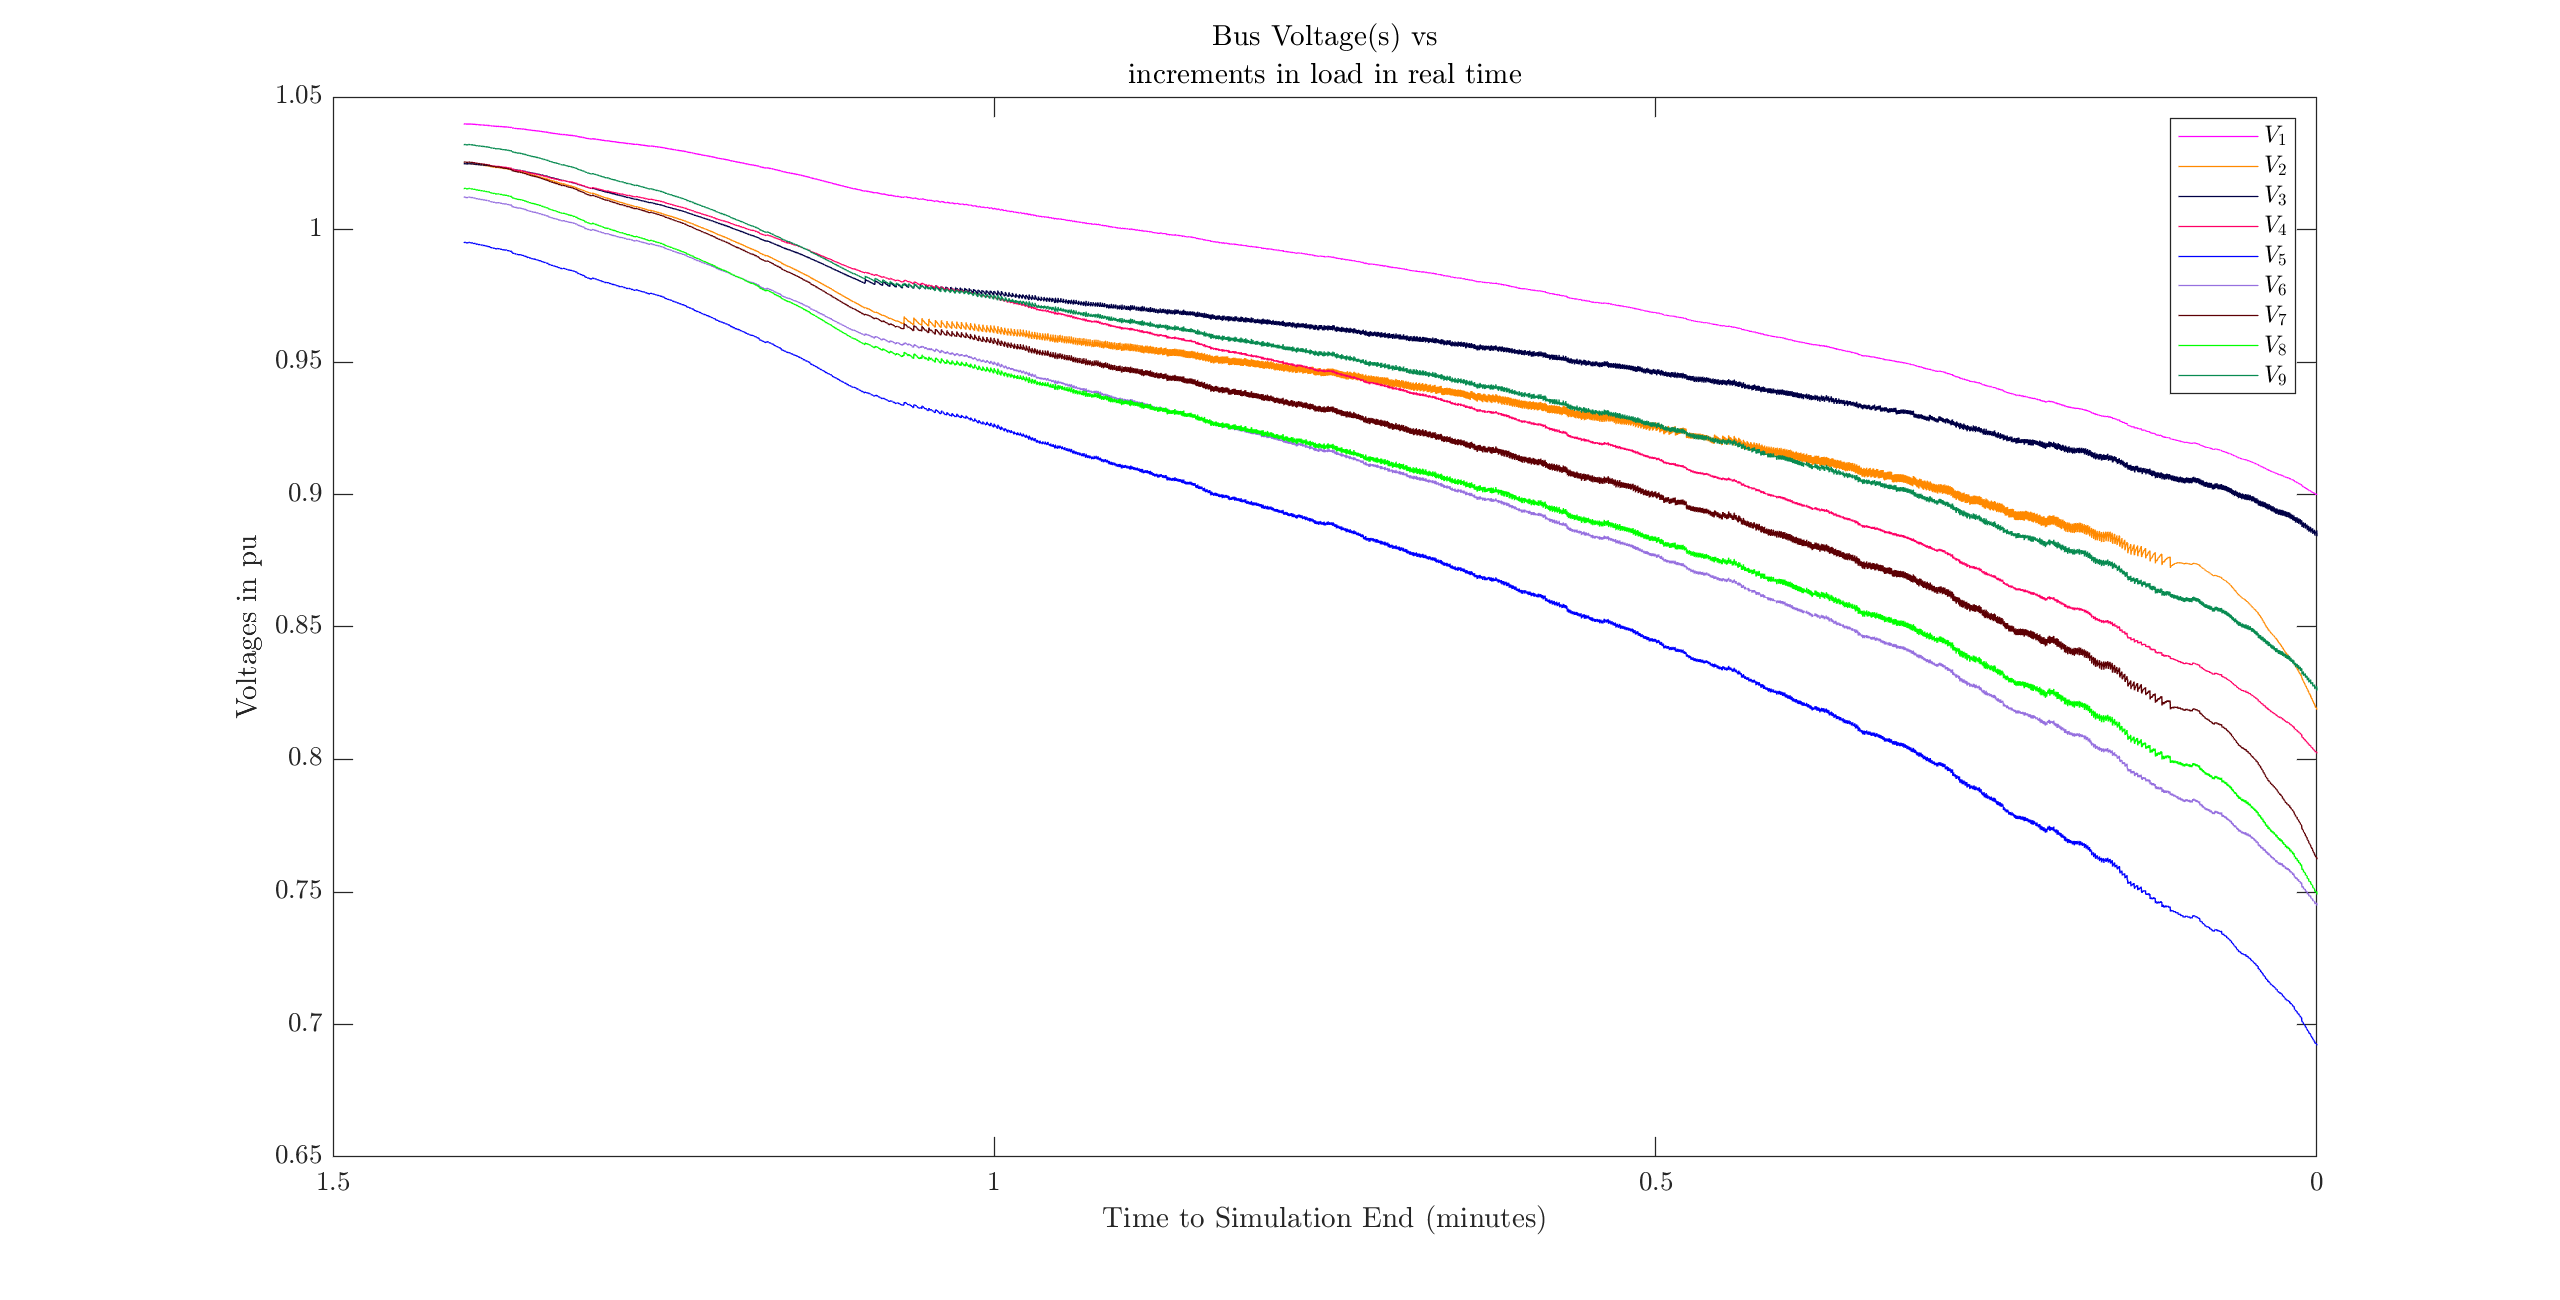
\includegraphics[scale=0.25]{../figures/analysis_matlab/voltages_run02}
		\caption{Bus Voltages for the simulated IEEE 9 Bus System vs simulation time.}
	\end{subfigure}

	\caption{Simulation results of the IEEE 9 Bus System as per the prescribed conditions.}
\end{figure}

\begin{figure}[!htpb]
	\begin{subfigure}{\textwidth}
		\centering
		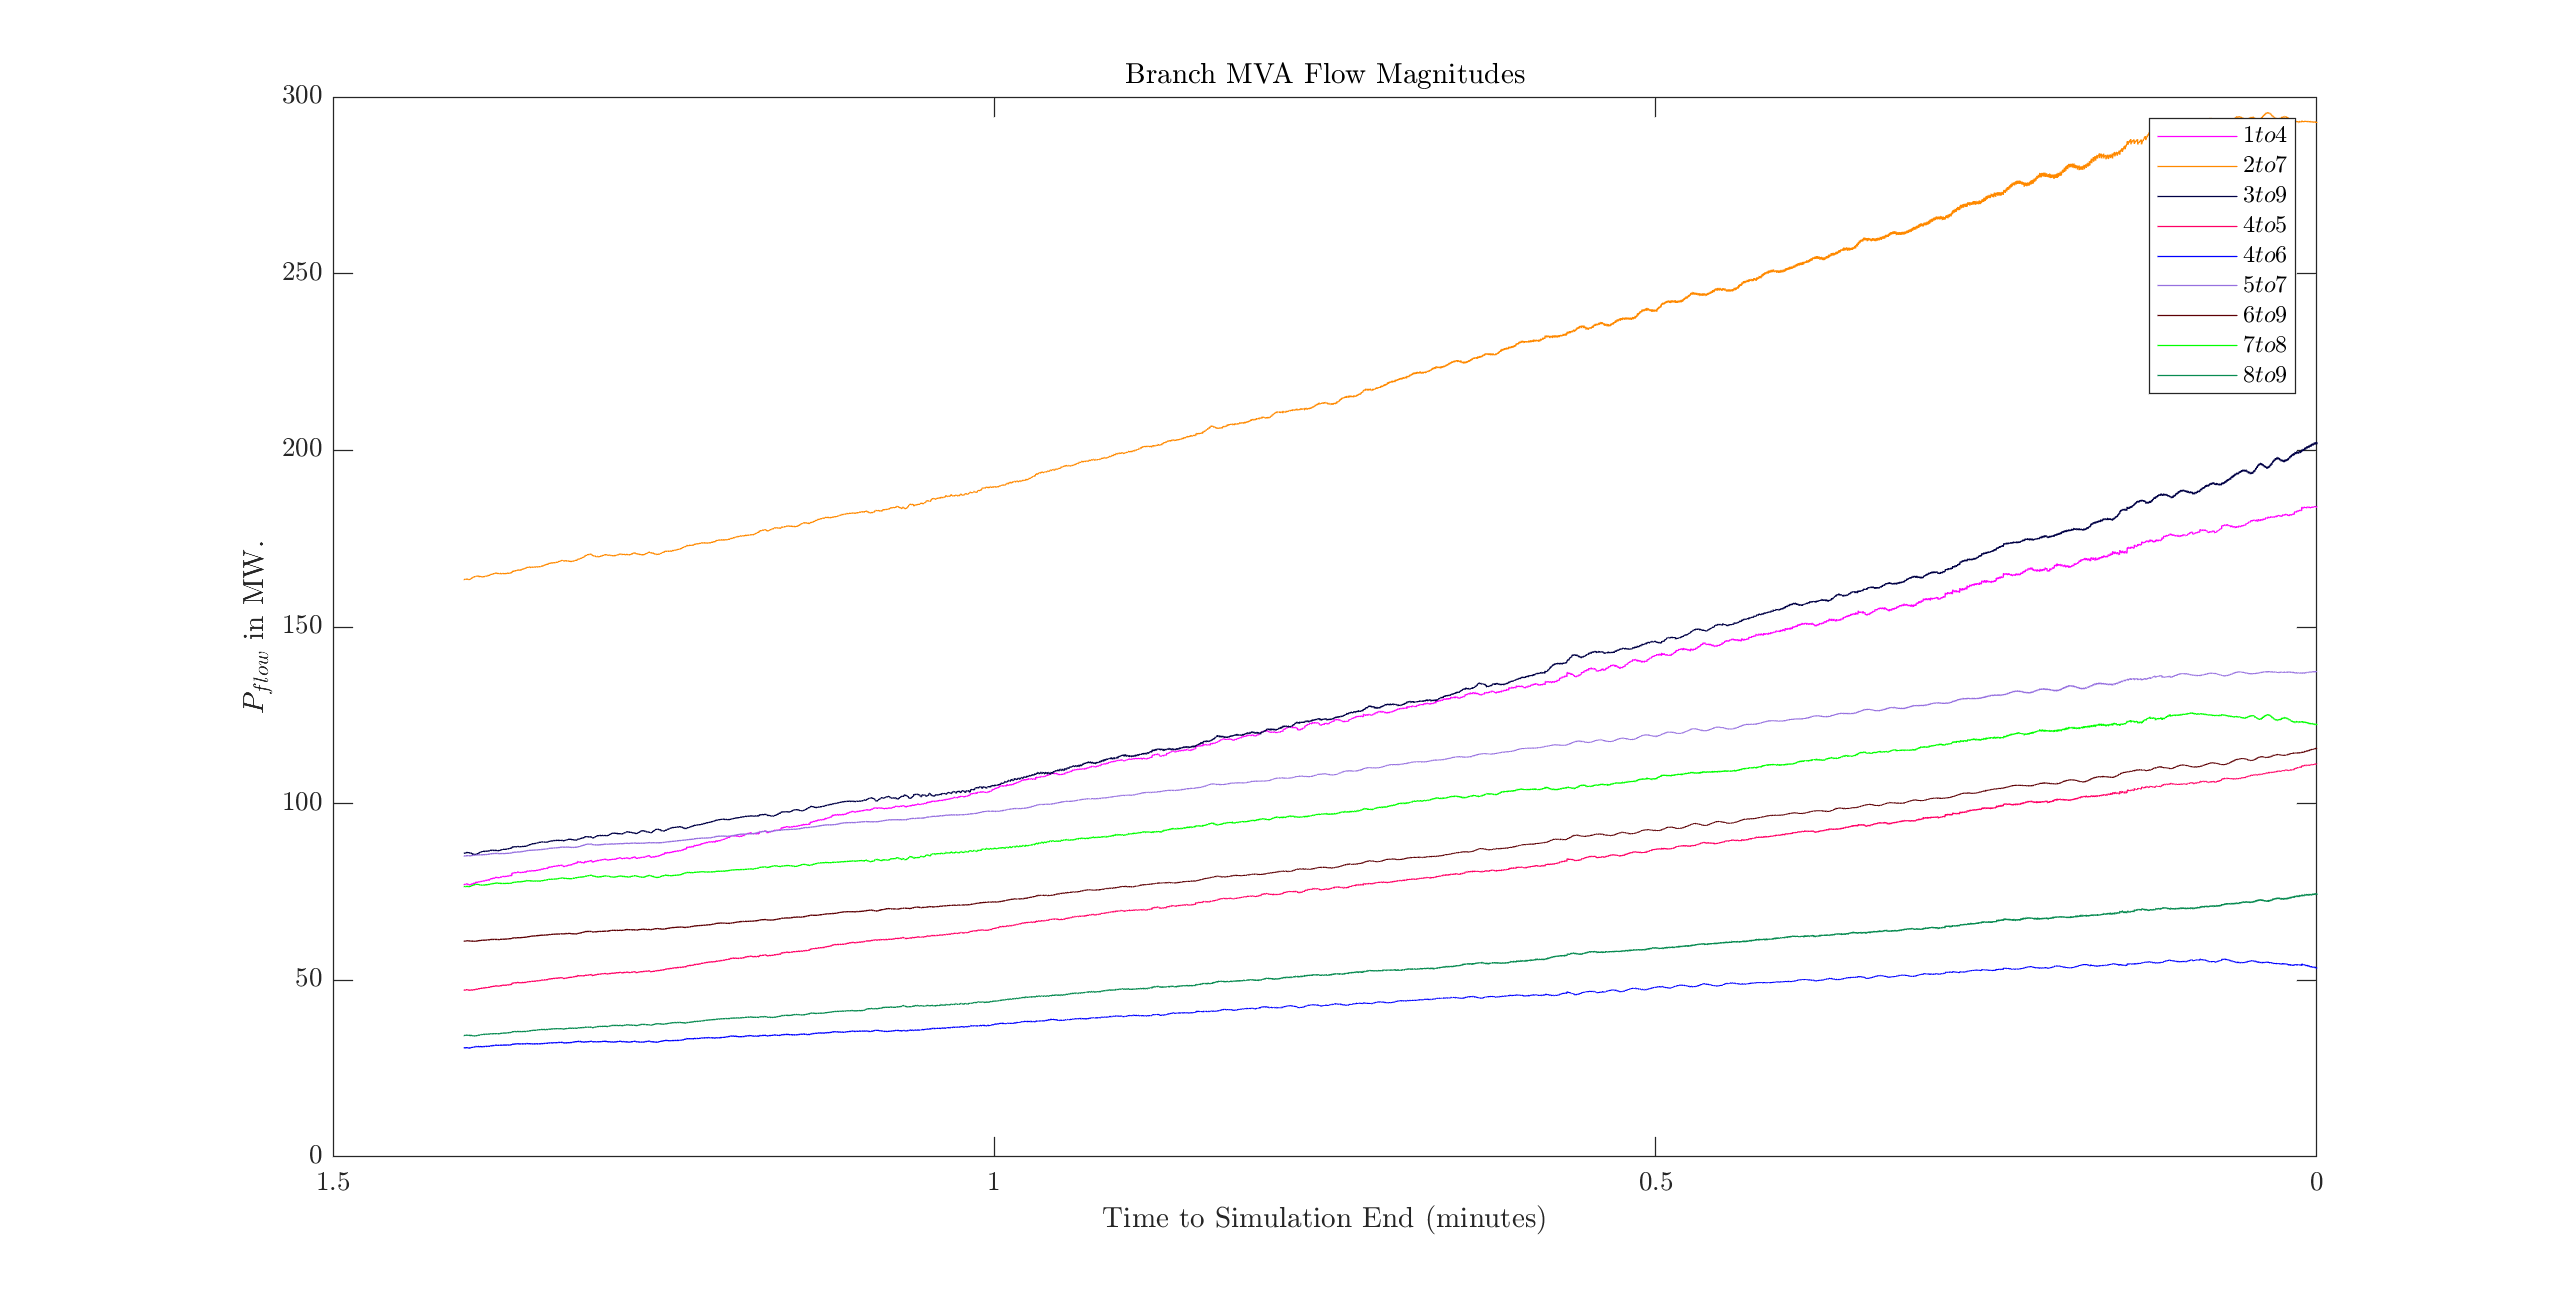
\includegraphics[scale=0.25]{../figures/analysis_matlab/currents_run02}
		\caption{Line Currents for the simulated IEEE 9 Bus System vs simulation time.}
	\end{subfigure}
	
	\begin{subfigure}{\textwidth}
		\centering
		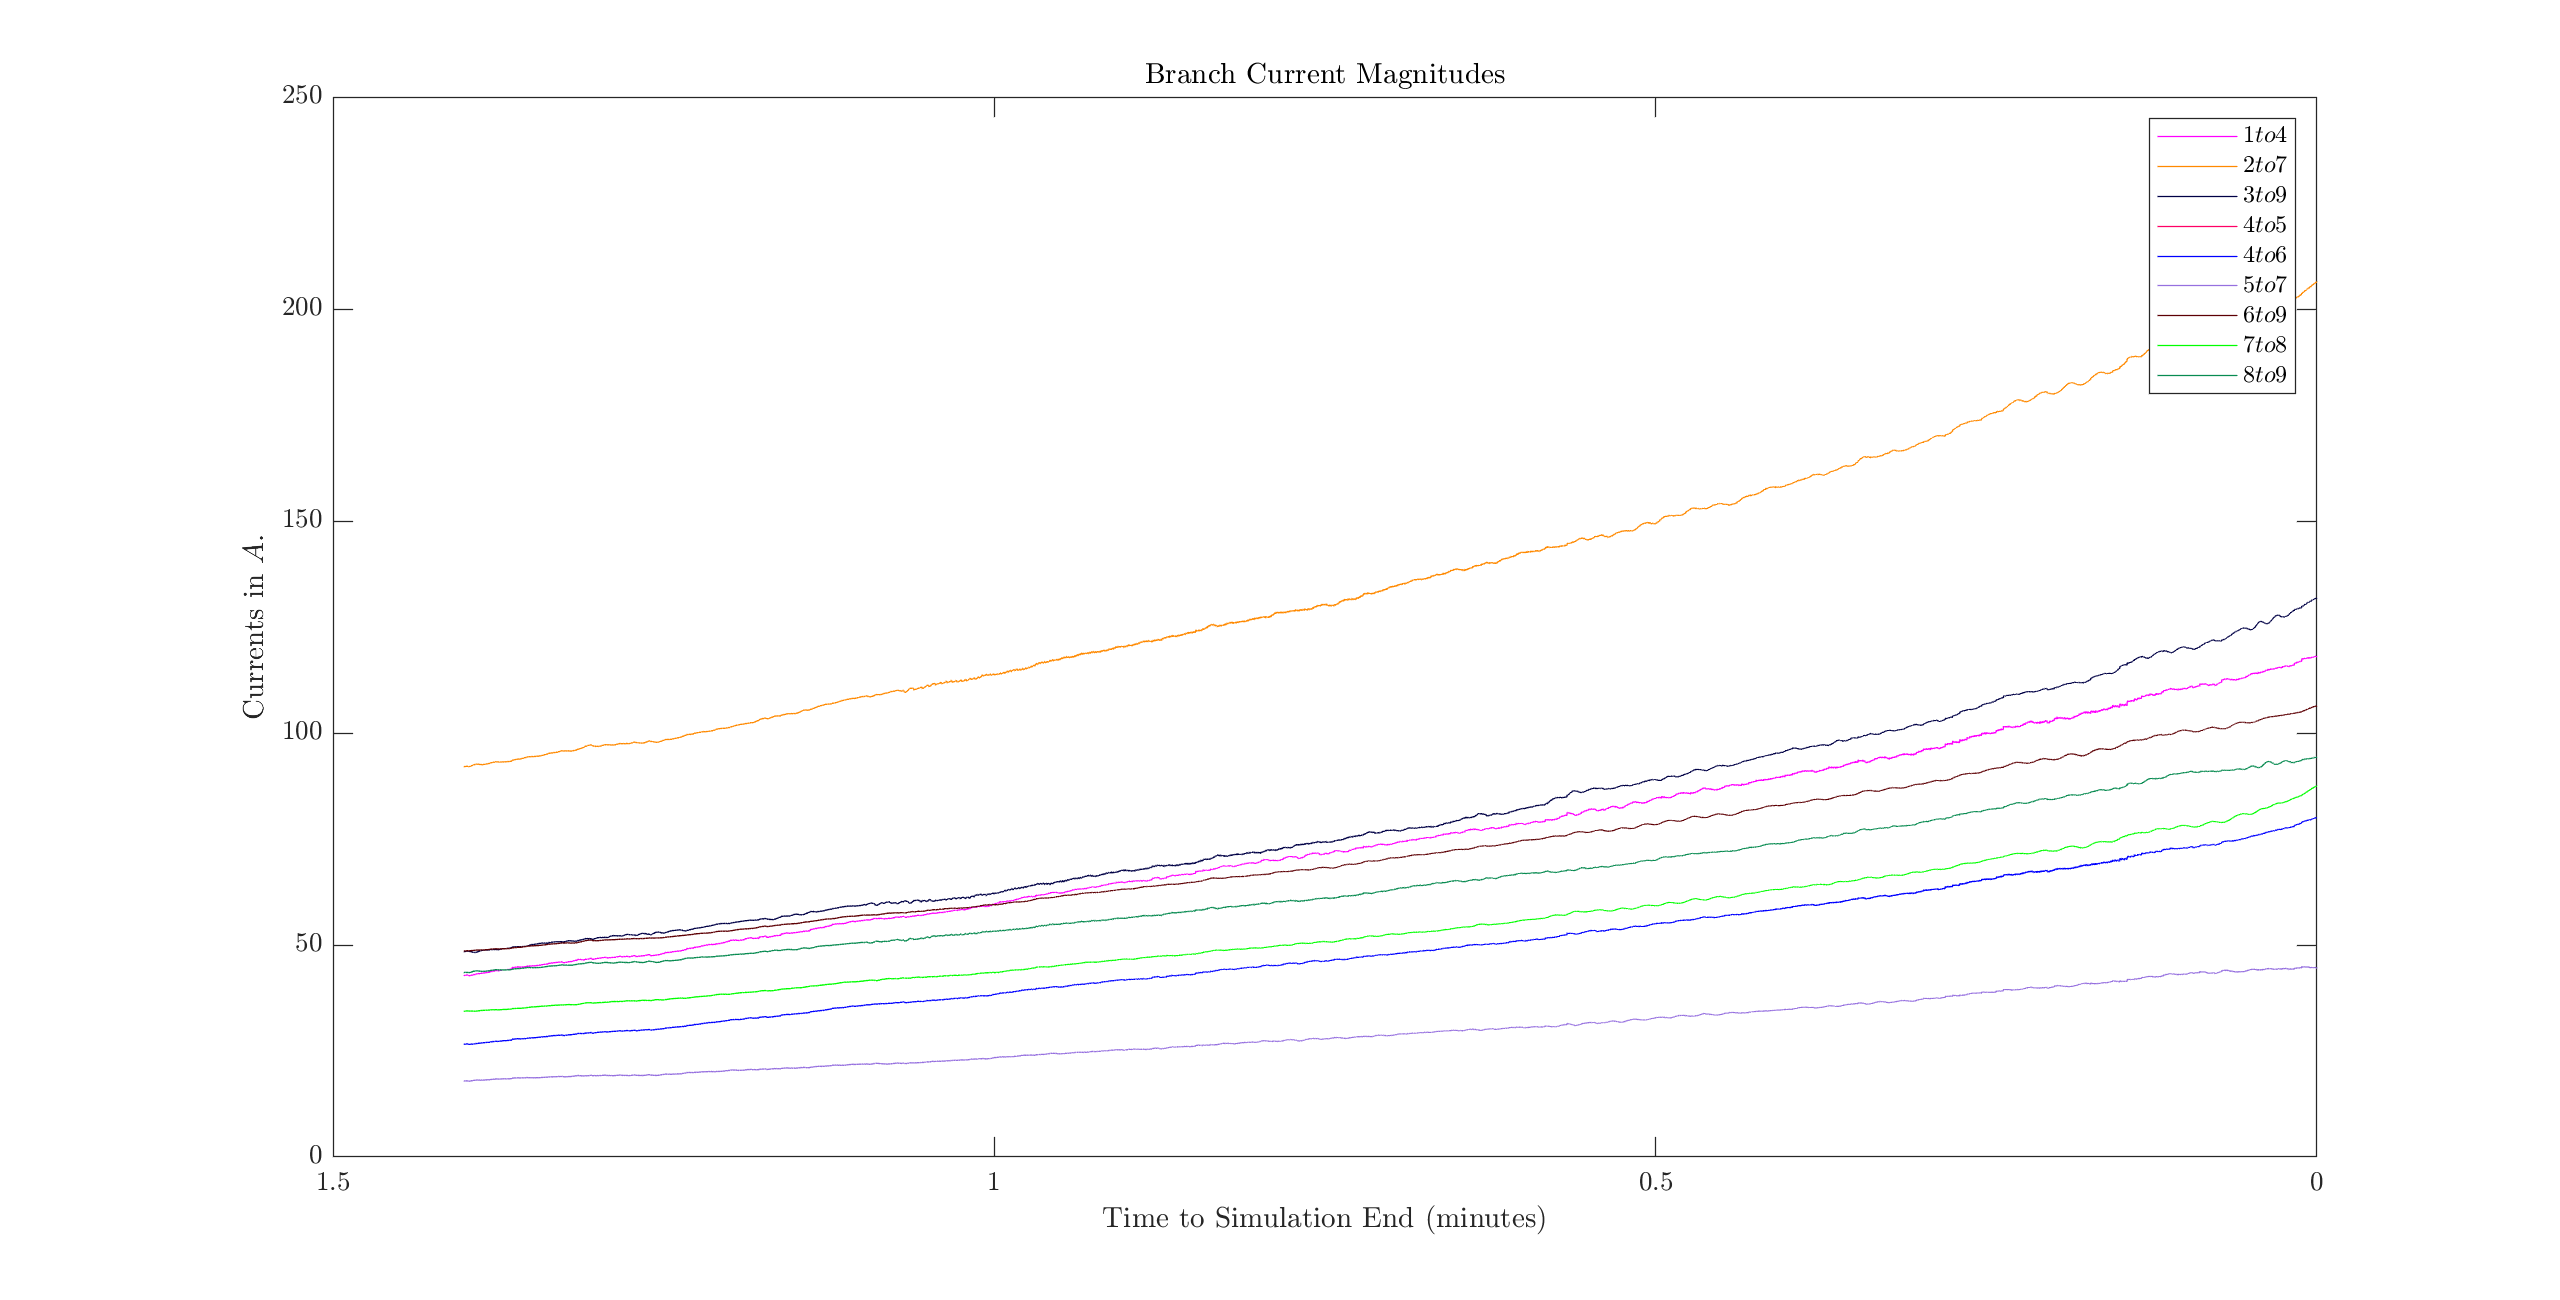
\includegraphics[scale=0.25]{../figures/analysis_matlab/mvas_run02}
		\caption{Line MVAs for the simulated IEEE 9 Bus System vs simulation time.}
	\end{subfigure}

	\caption{Simulation results of the IEEE 9 Bus System as per the prescribed conditions.}
\end{figure}

\clearpage
\textbf{Steps for Measuring Critical Slowing Down in the Simulation}

\begin{enumerate}
	\item Choosing a state variable to test for symptoms of Critical Slowing Down on. In this case, Bus Voltages were used to test the same. In the case of the IEEE 9 Bus system, the voltages were $V_1(t), V_2(t) \ldots V_9(t)$ in continuous-time or $V_1[n], V_2[n] \ldots V_9[n]$ in discrete-time.
	\item For real-time evaluation of a time-series in which the entire time-series is obviously unavailable at the current moment (unlike in the Offline Analysis), a running window of length $T$ seconds in real-time or alternatively $W$ instances in number of consecutive discrete-time readings of the chosen state variables (bus voltages) could be used for making analysis. In this thesis, $T=15$ seconds ($W=1500$ instances, as $W=\frac{T}{t_{sampling}}$ or $W=\frac{T}{f_{sampling}}$) was chosen.
	\item All instances of the bus voltages `covered' by the current window were:\\
		\begin{enumerate}
			\item Detrended via a Gaussian Kernel Smoothing function. \\
			Detrending a time-series, i.e. filtering out only the fluctuations in the time-series for analysis and rejecting the long-term slow trends is required for examining Critical Slowing Down as autocorrelation is meant for computation on detrended data, not on raw data, for effective analysis. The detrending was done by first passing the state variables (bus voltages) through a low pass filter, in this case, the Gaussian Kernel Smoothing filter and the resultant `smoothed' bus voltage signal were then subtracted from the original bus voltage signals.
			\begin{equation}
				GKS(n, \sigma_f) = \frac{1}{\sigma_f \sqrt{2\pi}}\exp{\left(-\frac{n^2}{2\sigma_f^2}\right)}
			\end{equation}
			where $\sigma_f$ is chosen in order to ascertain the bandwidth of the Low pass filter, such that only slow acting trends of the original bus voltage signals remain in the smoothed signals. In this case, $\sigma_f$ was taken to be 10.
			The detrended bus voltage signals were then obtained by subtracting the filtered signals from the original:
			\begin{equation}
				d(V_i[n]) = V_i[n] - GKS(V_i[n])
			\end{equation}
			\hspace{25pt} for the $i$th bus.
			The resultant detrended bus voltages may be viewed in Figure \ref{fig:detrendedBusVoltages}. 
			
			\item Subsequently, Fixed Lag Autocorrelation (with Lag $\tau = 1$ second) and Variance were computed over the detrended bus voltages. The autocorrelations were computed using \texttt{AR} function and variances were computed using the \texttt{var} function in MATLAB 2022a. Refer to Figure \ref{fig:autocorrAndVariance} for the results.
			
			\item Lastly, in order to statistically test for serial dependence of the autocorrelation and variance data (i.e. whether they are significantly increasing wrt time to be actually considered to be symptoms of Critical Slowing Down), a new kind of statistical parameter, namely the Modified Kendall's Tau Correlation Coefficient was computed over both of the previously computed Fixed Lag Autocorrelation and Variance values. In order to explain this new parameter, firstly the regular Kendall's Tau Correlation Coefficient is briefly introduced:
			\begin{equation}
				\label{eq:kenallsGeneral}
				\text{Kendall's } \tau = \frac{\text{Number of Concordant Pairs} - \text{Number of Discordant Pairs}}{\text{Total Number of Pairs}}
			\end{equation}
			\hspace{25pt} where, For a discrete-time series, such as $V_i[n]$ in the case of this thesis, a Concordant pair in a time series refers to two discrete-time instances $p$ and $q$ with $p<q$ such that $V_i[p] < V_i[q]$. Similarly, Discordant pairs refer to the cases where $V_i[p] > V_i[q]$. Note that $i$ only refers to the bus number in the IEEE 9 Bus System. \\
			Kendall's Tau Correlation Coefficient is valued between $-1$ and $1$, but also has an associated p-value, which measures the confidence of the null hypothesis that the serial dependence of a time-series is statistically significant. Sometime, the p-value is not statistically significant (p-value > 0.05) but applying Kendall's Test still outputs a correlation coefficient value, making the test equivocal. Thus to accommodate for the confidence interval along with the obtained correlation coefficients, a new parameter for testing the serial dependence of data, namely the Modified Kendall's Tau Correlation Coefficient (or MKTCC in short) was used to test if the increases in Fixed Lag Autocorrelations and Variances were statistically significant:
			\begin{equation}
				\label{eq:mktccAutocorrAndVariance}
				\text{Modified Kendall's } \tau' = -\tau \log{(\text{pVal}_{\tau})}
			\end{equation}
			In Figure \ref{fig:mktccAutocorrAndVariance}, it can be observed how the MKTCC value of their autocorrelation and variance values shoot up faster than those of others. While in this thesis, this observation was not continued with in a rigorous quantitative analysis, this statistical parameter seems promising as an early warning sign indicator of proximity to instability for a power grid, and identifying areas in the grid which are the most vulnerable to instabilities caused by steadily increasing stochastic variations in load.
		\end{enumerate}
	
	\item Next the window is moved by a length equivalent to $T_{moving}$ seconds or $W_{moving}$ discrete time instances. In this case, $T_{moving} = T/10$ or $T_{moving} = 1.5$ seconds (and therefore $W_{moving} = 150$ discrete-time instances).
	
	\item Goto Step 3 until simulation ends.
\end{enumerate}

\begin{figure}[!htpb]
	\centering
	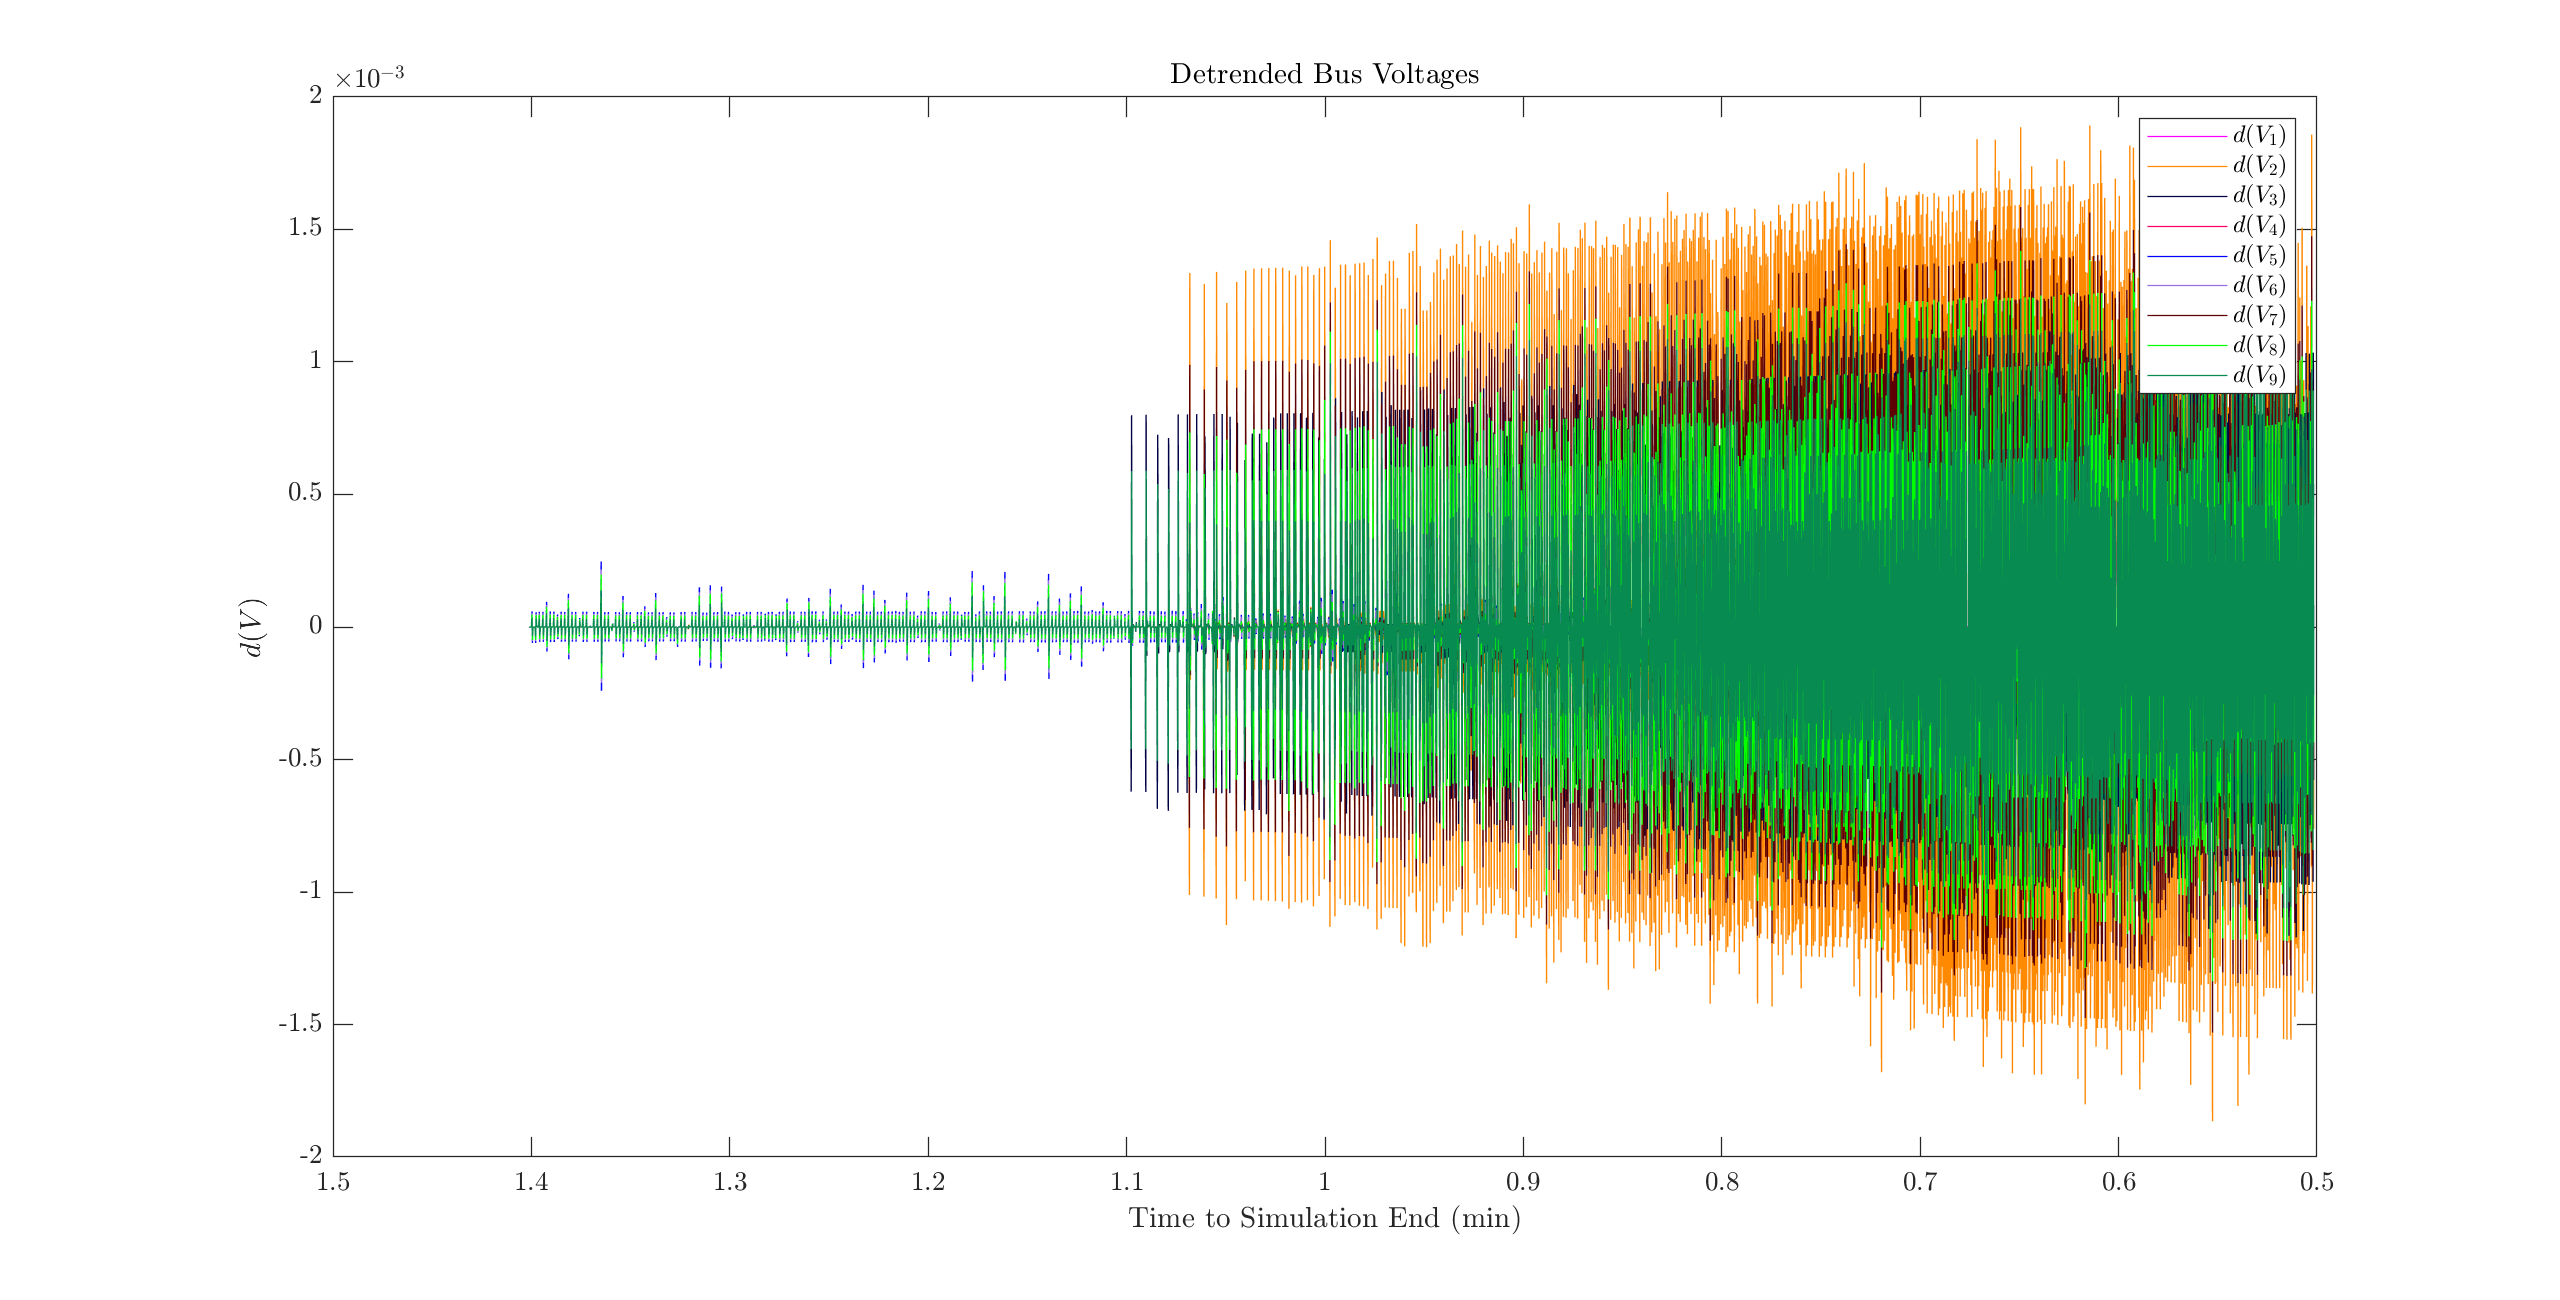
\includegraphics[scale=0.25]{../figures/analysis_matlab/voltsDetrended_run02}
	\caption{Detrended Bus Voltages for the simulated IEEE 9 Bus System vs simulation time.}
	\label{fig:detrendedBusVoltages}
\end{figure}

\begin{figure}[!htpb]
	\begin{subfigure}{\textwidth}
		\centering
		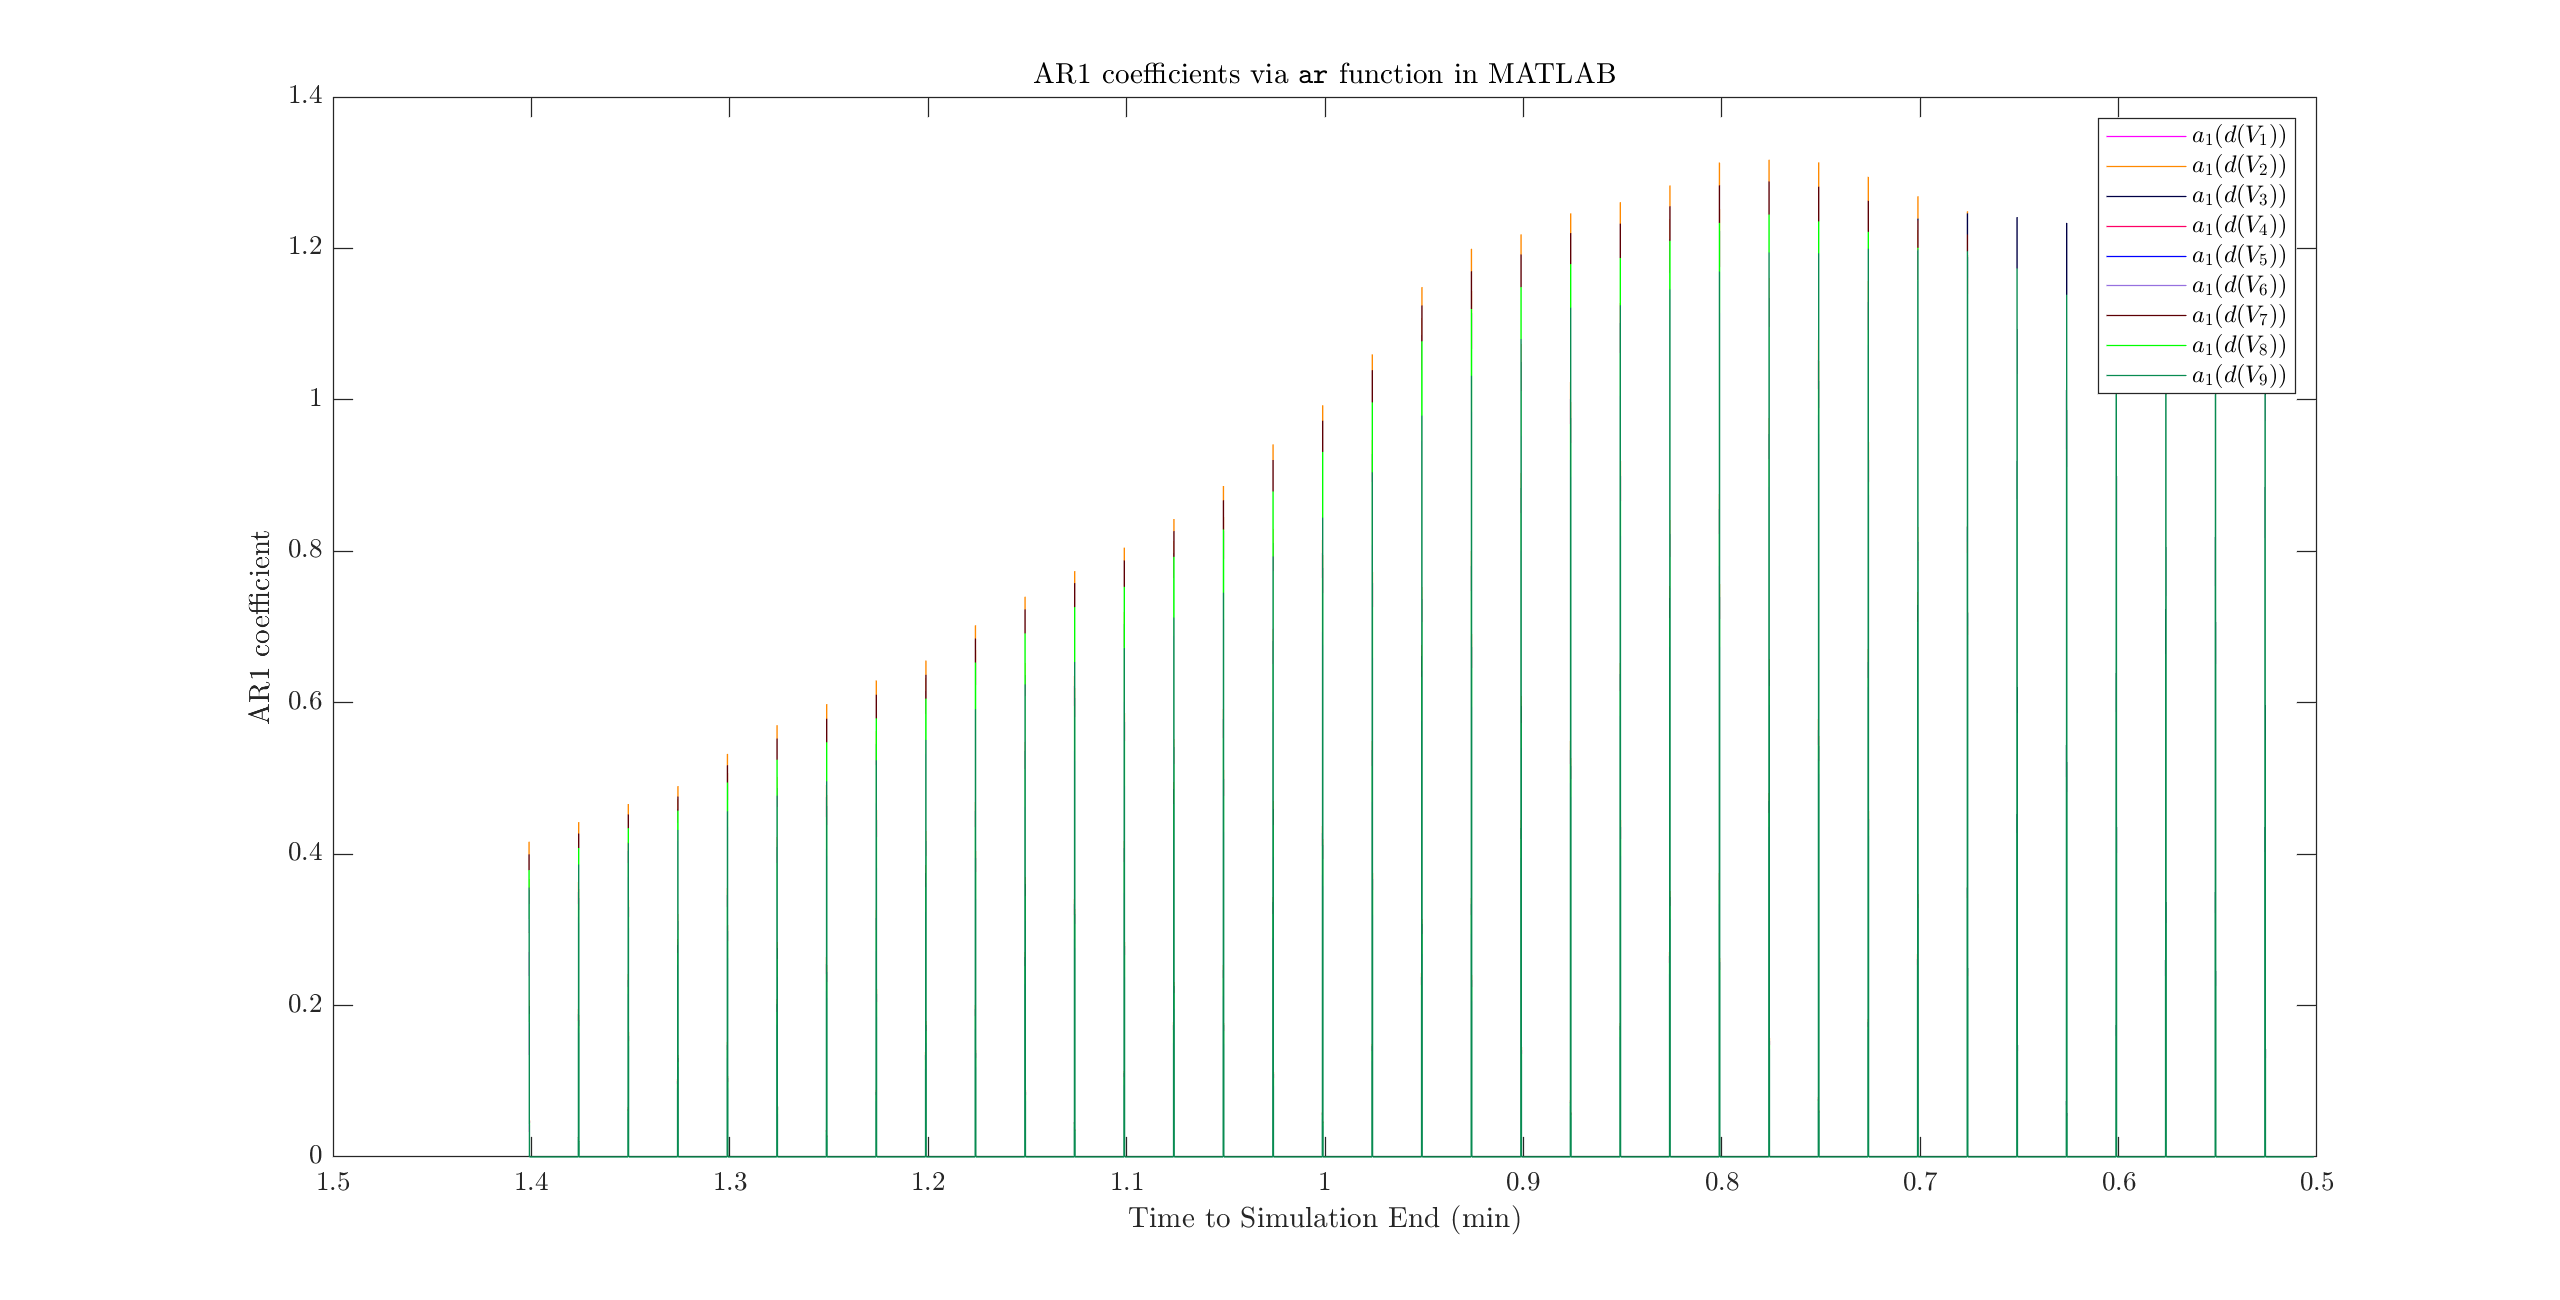
\includegraphics[scale=0.25]{../figures/analysis_matlab/ar1_run02}
		\caption{Fixed Lag Autocorrelations (un-normalized) with Lag $\tau = 1s$ computed for the Detrended Bus Voltages for the simulated IEEE 9 Bus System vs simulation time.}
	\end{subfigure}
	
	\begin{subfigure}{\textwidth}
		\centering
		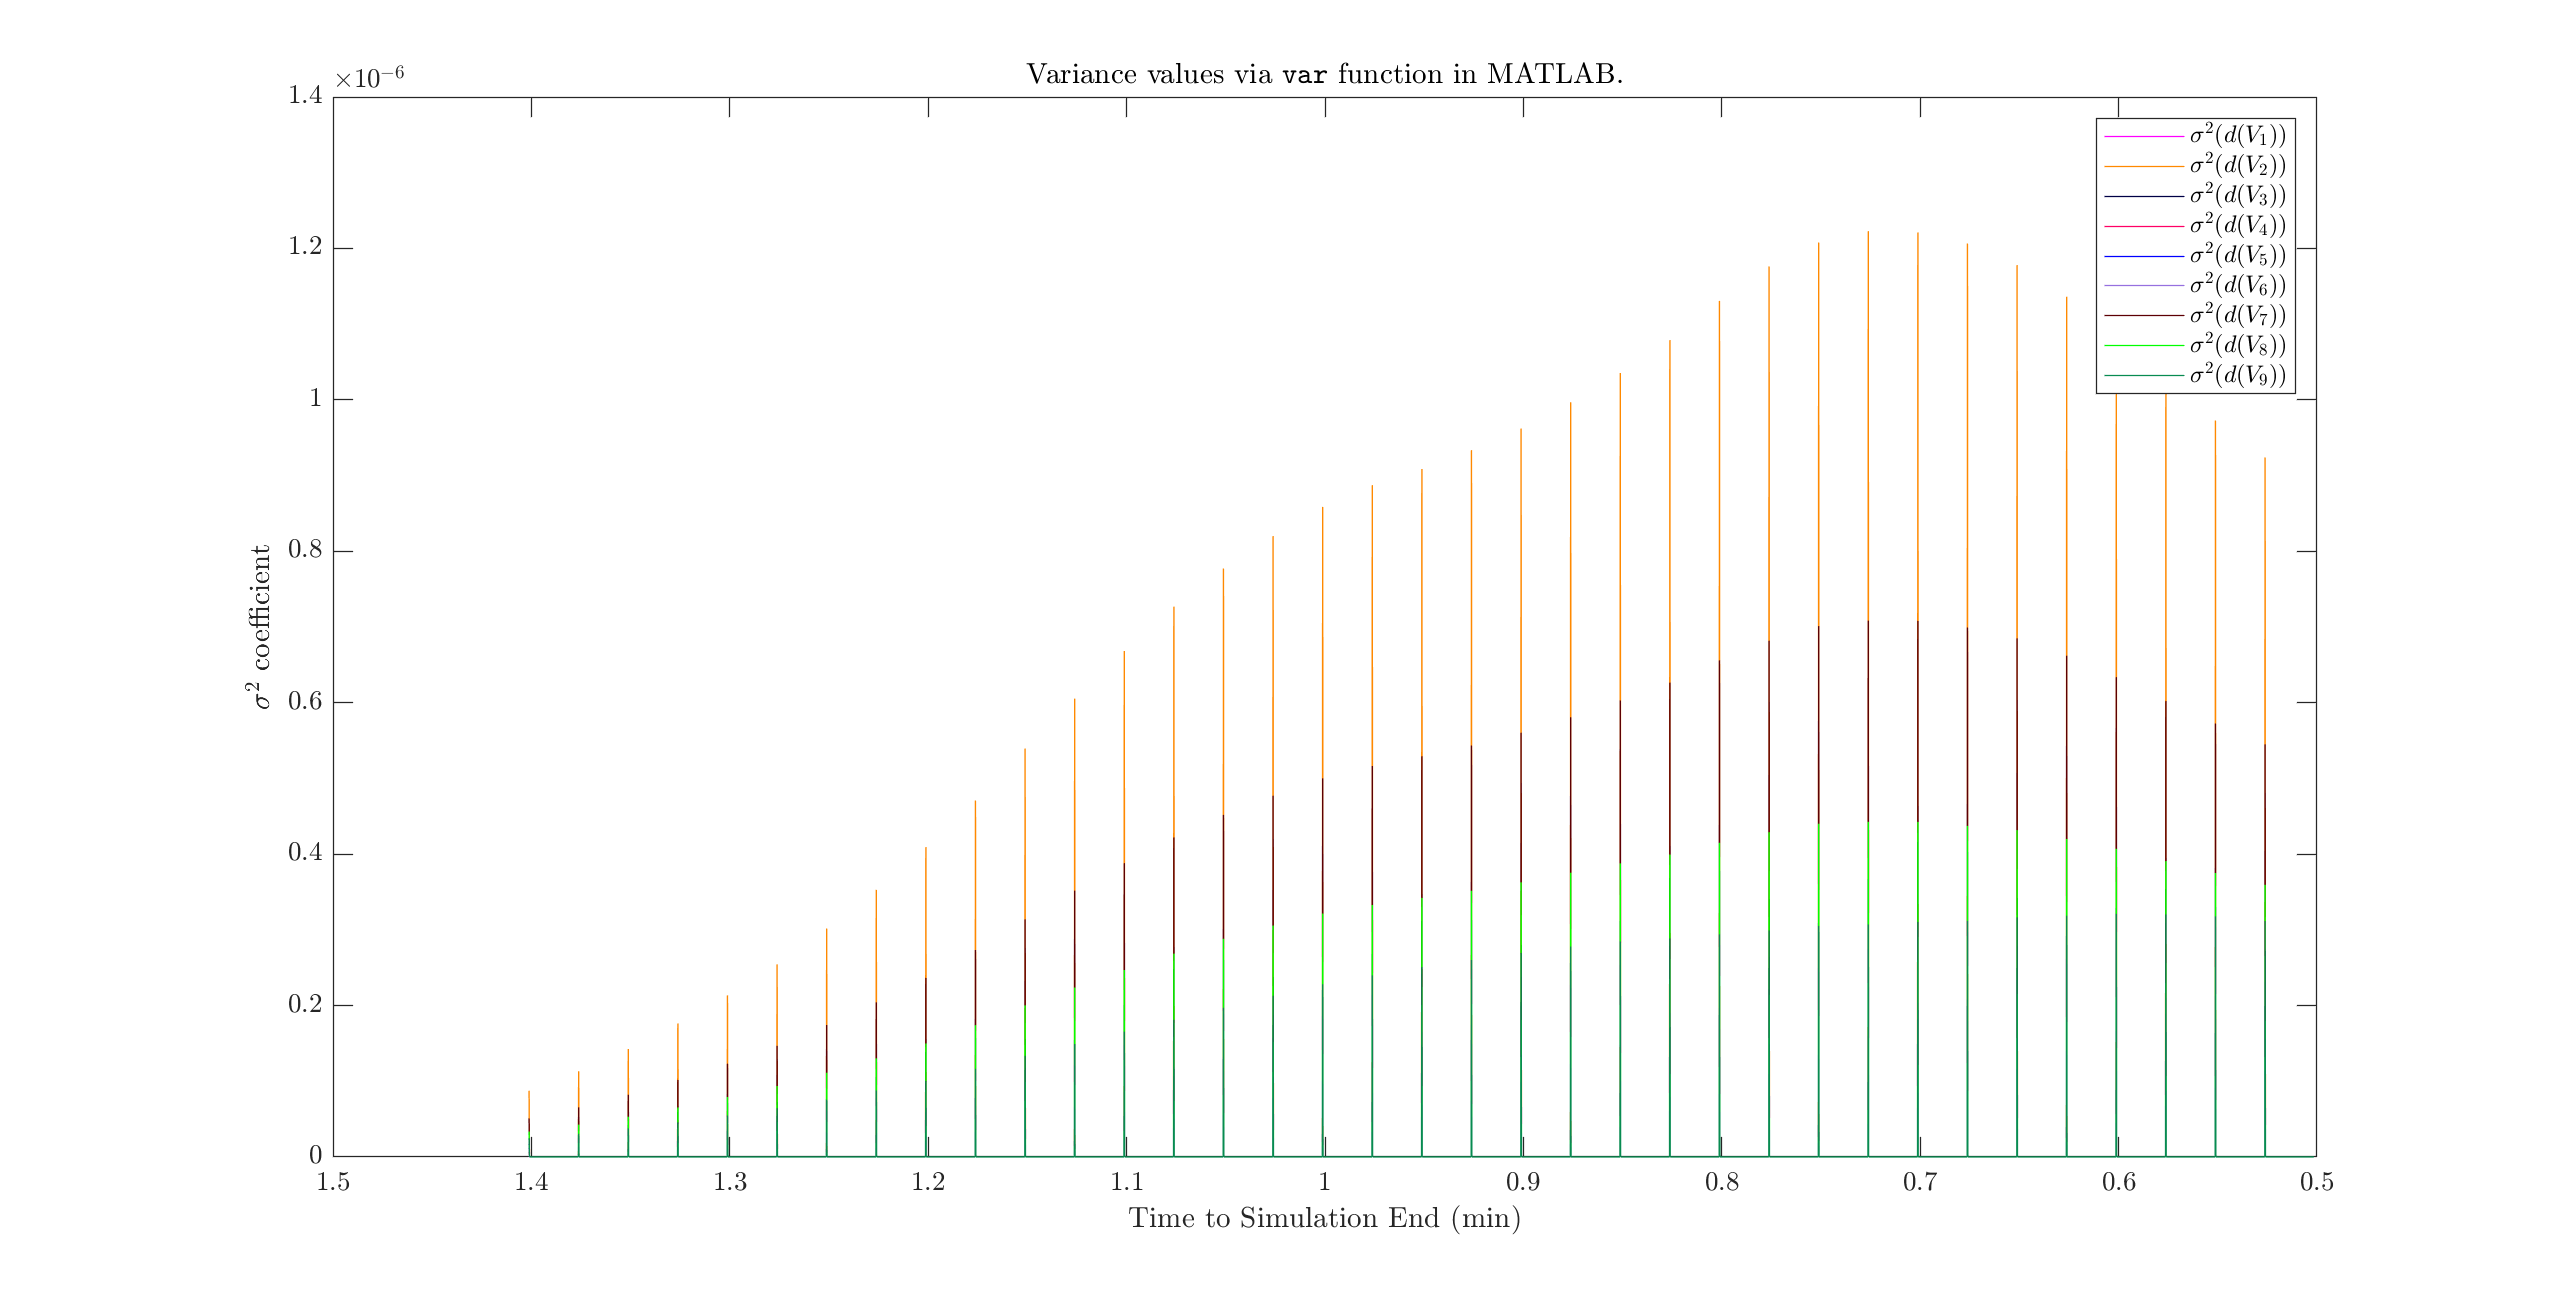
\includegraphics[scale=0.25]{../figures/analysis_matlab/var_run02}
		\caption{Variances computed for the Detrended Bus Voltages for the simulated IEEE 9 Bus System vs simulation time.}
	\end{subfigure}
	
	\caption{Data Analysis done on the Bus Voltages resulting from the IEEE 9 Bus System Simulation for the purpose of testing if the system shows symptoms of Critical Slowing Down.}
	\label{fig:autocorrAndVariance}
\end{figure}

\begin{figure}[!htpb]
	\begin{subfigure}{\textwidth}
		\centering
		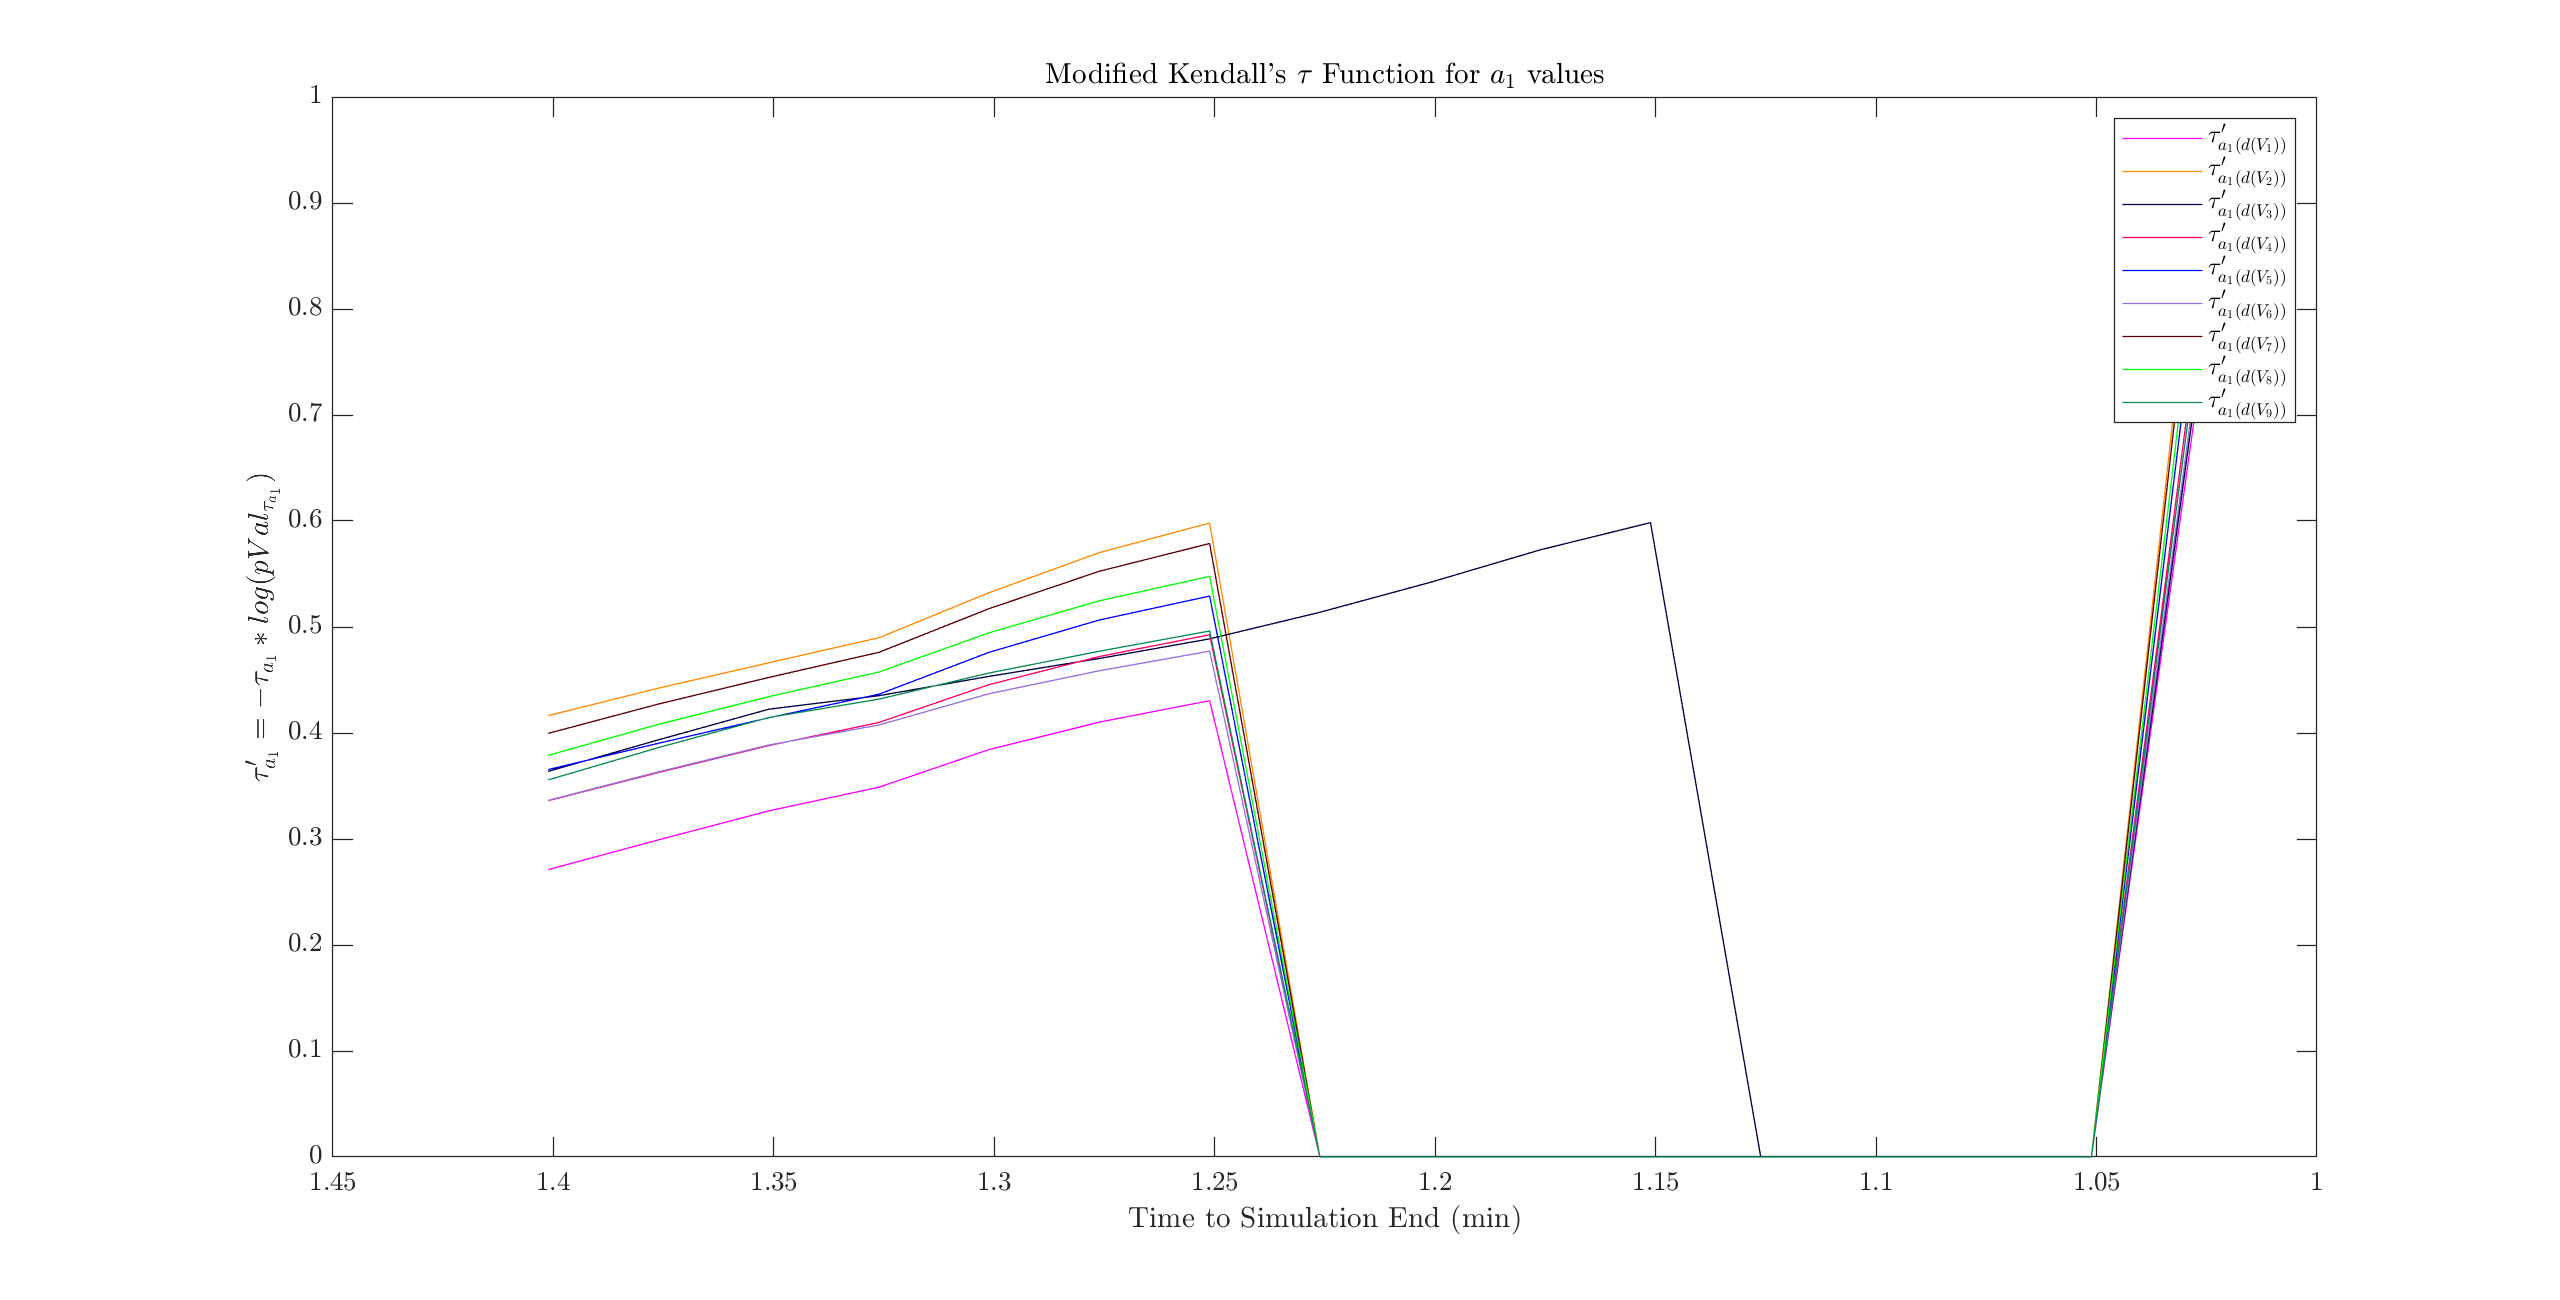
\includegraphics[scale=0.25]{../figures/analysis_matlab/mktcc_ar1_run02}
		\caption{Modified Kendall's Tau Correlation Coefficients (MKTCC) computed for the previously computed Fixed Lag Autocorrelations of the Detrended Bus Voltages.}
	\end{subfigure}
	
	\begin{subfigure}{\textwidth}
		\centering
		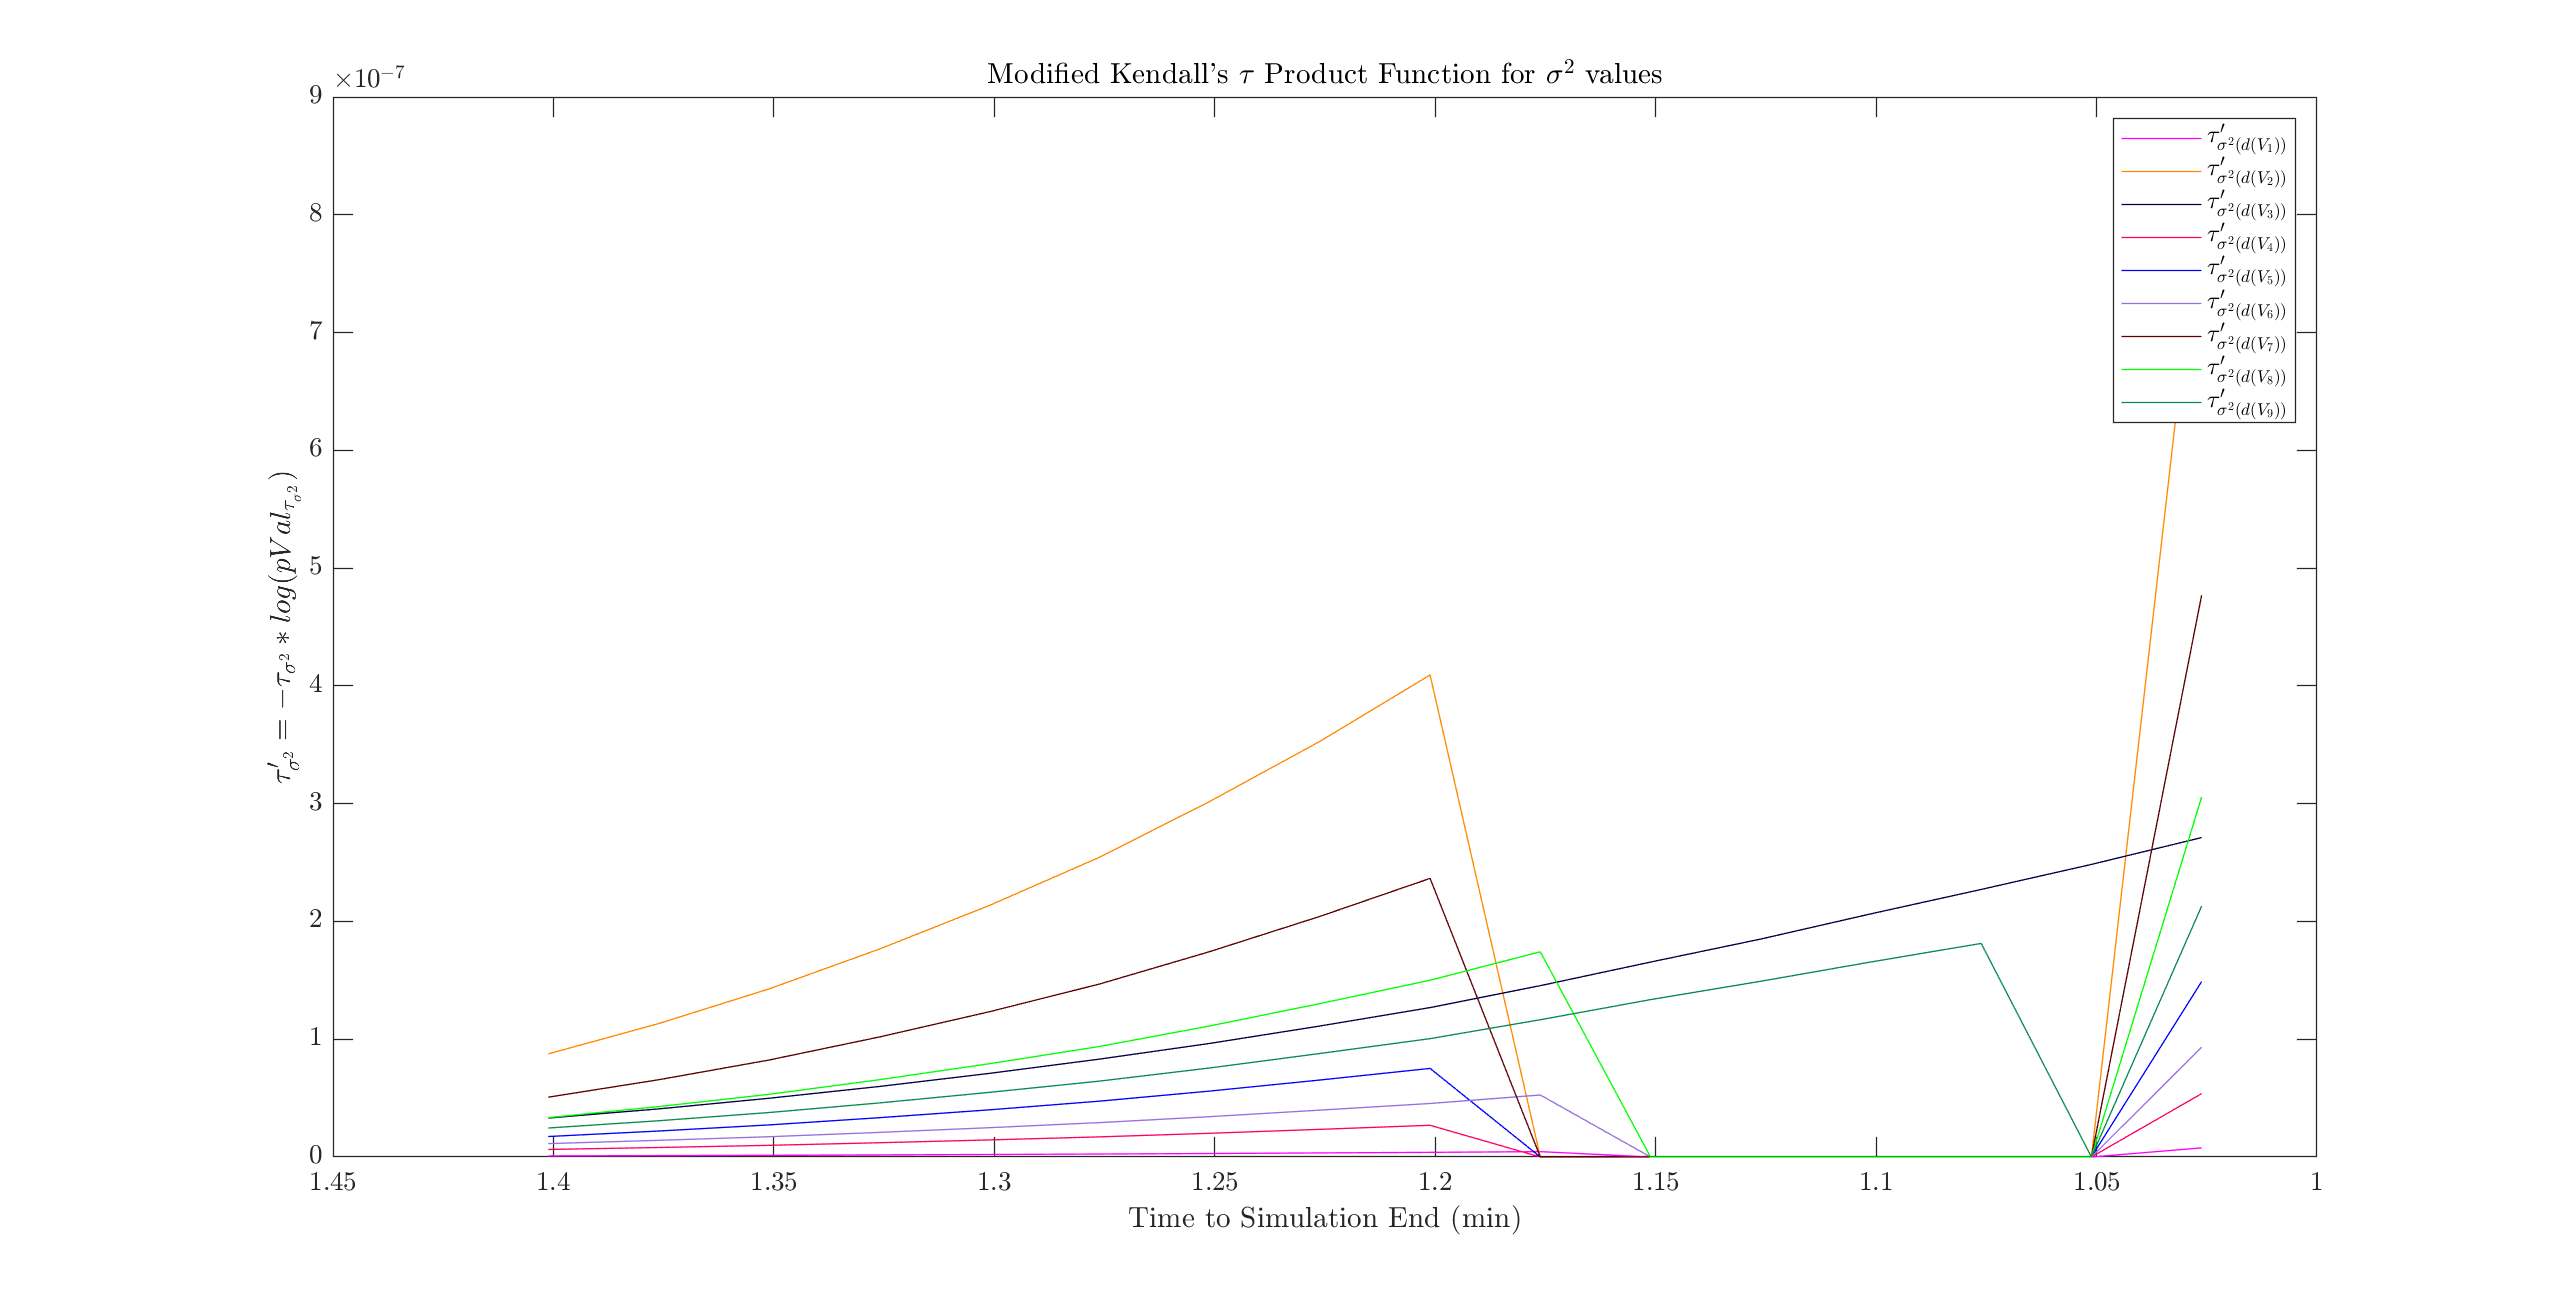
\includegraphics[scale=0.25]{../figures/analysis_matlab/mktcc_var_run02}
		\caption{Modified Kendall's Tau Correlation Coefficient (MKTCC) computed for the previously computed Variances of the Detrended Bus Voltages.}
	\end{subfigure}
	
	\caption{Modified Kendall's Tau Correlation Coefficient was used for checking for any serial dependence of the autocorrelation and variance data, i.e. if the increases in both parameters was statistically significant or not.}
	\label{fig:mktccAutocorrAndVariance}
\end{figure}

\clearpage
Continuous stress on the power grid in the form of a constantly increasing power demand on the generators is bound to cause a blackout in the grid. In simulation terms, this is when the `Network Not Converged' error message is thrown by PSSE, and in mathematical terms, this phenomenon is called as Critical Bifurcation.
It was verified using visual inspection of the Fixed Lag Autocorrelation plots, Variance plots and their respective Modified Kendall's Tau Correlation Coefficient plots that Fixed Lag Autocorrelation and Variance of Bus Voltages are suitable early warning signs for indicators to instability in the power grids, predicting the critical bifurcation event a minute earlier. It may be noted that the time by which an advanced prediction of an impending critical bifurcation is does not carry much meaning without accommodating the size of the grid and the degree of load demand stress on the grid. Other simulations were done with lower stress (~5\% to 7\% increase in demand power per minute) whose analysis would lead to an earlier prediction of the impending critical bifurcation (around several minutes before the event). Similarly, a higher stress (~25\% per minute) could only be diagnosed around thirty seconds earlier.
Ultimately, the figure of interest is the ratio of the time of prediction made vs the total simulation time. In all instances, the prediction was made at the latest, half-way through the simulation. This implies that the algorithm is appropriate to diagnose proximity to instabilities in a power grid before any harm is done. 

Lastly, it should be noted that while autocorrelation was used in both online/real-time (as Fixed Lag Autocorrelation) and offline/postmortem analyses (as Fixed Time Autocorrelation), the two usages were different in:

\begin{itemize}
	\item their mode of procuring and processing input data (a running window of an incoming stream of data vs previously stored months/years worth of time series),
	\item the degrees of freedom allowed for its two parameter variables (which out of $t$ and $\tau$ is allowed to be constant),
	\item their theoretically expected output data (autocorrelation is should decrease exponentially with respect to time lag $\tau$ but increase with time $t$ if that the system is being progressively stressed with time)
\end{itemize} 
 
 